\documentclass[10pt,journal,compsoc]{IEEEtran}

\usepackage{alltt}
\usepackage{multirow}
\usepackage{graphicx}
\usepackage{color}
\usepackage[labelfont=bf,textfont={bf}]{caption}
\usepackage{subcaption}
\usepackage{pifont}% http://ctan.org/pkg/pifont
\usepackage{boxedminipage}
\usepackage{flushend}
\usepackage{notoccite}
\usepackage{array}
\newcolumntype{C}[1]{>{\centering\let\newline\\\arraybackslash\hspace{0pt}}m{#1}}
\usepackage{booktabs}
\usepackage[framemethod=tikz]{mdframed}
\usepackage{lipsum}
\usetikzlibrary{shadows}
\usepackage{mathtools}
 \usepackage{paralist}
 \definecolor{light-gray}{gray}{0.80}
\usepackage{graphics}
\newmdenv[
tikzsetting= {fill=light-gray},
linewidth=1pt,
roundcorner=0pt, 
shadow=false
]{myshadowbox}
\usepackage{colortbl} 
\usepackage{subcaption}
% \usepackage[shortlabels]{enumerate}
\usepackage{blindtext, graphicx}
\usepackage{textcomp}
\usepackage{mathtools}
\usepackage{hyperref}
\usepackage{amsmath}
\usepackage{amsfonts}
\usepackage{caption}
\usepackage{color}
\usepackage[final]{listings}
\usepackage{graphicx} 
\usepackage{multirow}
\usepackage{balance}
\usepackage{picture}
\usepackage{relsize}
\usepackage{soul}
\usepackage{enumitem}
\setitemize{noitemsep,topsep=0pt,parsep=0pt,partopsep=0pt}
\DeclarePairedDelimiter\abs{\lvert}{\rvert}%
%\usepackage{mathptmx} \usepackage[scaled=.90]{helvet} \usepackage{courier}
%\usepackage{fourier} 
\usepackage{array}
\usepackage{makecell}

\newcommand{\tion}[1]{\S\ref{sect:#1}}
\newcommand{\fig}[1]{Fig.~\ref{fig:#1}}
\newcommand{\tab}[1]{Tab.~\ref{tab:#1}}

\definecolor{comment_color}{rgb}{0.5, 0, 1}
\renewcommand\theadalign{cb}
\renewcommand\theadfont{\bfseries}
\renewcommand\theadgape{\Gape[4pt]}
\renewcommand\cellgape{\Gape[4pt]}


\newcommand{\cmark}{\ding{51}}%
\newcommand{\xmark}{\ding{55}}%

\newcommand{\todoc}[2]{{\textcolor{#1}{\textbf{[[#2]]}}}}
\newcommand{\todobrown}[1]{\todoc{green}{\textbf{[[#1]]}}}
\newcommand{\todoblue}[1]{\todoc{blue}{\textbf{[[#1]]}}}
\newcommand{\todoorange}[1]{\todoc{cyan}{\textbf{[[#1]]}}}
\newcommand{\todored}[1]{\todoc{red}{\textbf{[[#1]]}}}


\newcommand{\bi}{\begin{itemize}}
\newcommand{\ei}{\end{itemize}}
% Set letter paper size:
\setlength{\paperheight}{11in}
\setlength{\paperwidth}{8.5in}
\usepackage[
  pass,% keep layout unchanged
  % showframe,% show the layout
]{geometry}
\usepackage{verbatim}
\usepackage{algorithm}
\usepackage{algorithmicx}
\usepackage{algpseudocode}
\usepackage[export]{adjustbox}
\usepackage{mathtools}
\setlength{\belowcaptionskip}{-10pt}
\renewcommand{\footnotesize}{\scriptsize}
\definecolor{lightgray}{gray}{0.8}
\definecolor{darkgray}{gray}{0.6}
\renewcommand{\algorithmicrequire}{\textbf{Input:}}
\renewcommand{\algorithmicensure}{\textbf{Output:}}
\definecolor{Gray}{rgb}{0.88,1,1}
\definecolor{Gray}{gray}{0.85}
\definecolor{Blue}{RGB}{0,29,193}
\definecolor{MyDarkBlue}{rgb}{0,0.08,0.45} 
\lstset{
    language=Python,
    basicstyle=\sffamily\fontsize{2.5mm}{0.8em}\selectfont,
    breaklines=true,
    prebreak=\raisebox{0ex}[0ex][0ex]{\ensuremath{\hookleftarrow}},
    frame=l,
    showtabs=false,
    columns=fullflexible,
    showspaces=false,
    showstringspaces=false,
    keywordstyle=\bfseries\sffamily\fontsize{2.8mm}{0.6em},
    emph={progressive, build_model, rank_based, projective, measure, acquisition_function, stopping_criterion, recombine, selector, init_population, EA, SWAY, cluster, split, BayesianOpt, ePAL, GO, model_predict, discard, get_next_point, predict, non_dominated_sort, assign_cdom_scores, FLASH, acquisition_fn, Bazza }, emphstyle=\bfseries\color{blue!50!black},
    stringstyle=\color{green!50!black},
    commentstyle=\color{red!50!black}\it,
    numbers=left,
    captionpos=t,
    escapeinside={\%*}{*)}
}


\usepackage{fancyvrb}
\fvset{%
fontsize=\small,
numbers=left
}

\newcommand{\be}{\begin{enumerate}}
\newcommand{\ee}{\end{enumerate}}
\newcommand{\eq}[1]{Equation~\ref{eq:#1}}

%%% graph
\newcommand{\crule}[3][darkgray]{\textcolor{#1}{\rule{#2}{#3}}}
%\newcommand{\rone}{\crule{1mm}{1.95mm}}
%\newcommand{\rtwo}{\crule{1mm}{1.95mm}\hspace{0.3pt}\crule{1mm}{1.95mm}}
%\newcommand{\rthree}{\crule{1mm}{1.95mm}\hspace{0.3pt}\crule{1mm}{1.95mm}\hspace{0.3pt}\crule{1mm}{1.95mm}}
%\newcommand{\rfour}{\crule{1mm}{1.95mm}\hspace{0.3pt}\crule{1mm}{1.95mm}\hspace{0.3pt}\crule{1mm}{1.95mm}\hspace{0.3pt}\crule{1mm}{1.95mm}} 
%\newcommand{\rfive}{\crule{1mm}{1.95mm}\hspace{0.3pt}\crule{1mm}{1.95mm}\hspace{0.3pt}\crule{1mm}{1.95mm}\hspace{0.3pt}\crule{1mm}{1.95mm}}
\newcommand{\quart}[3]{\begin{picture}(80,6)%1
{\color{black}\put(#3,3){\circle*{4}}\put(#1,3){\line(1,0){#2}}}\end{picture}}
\newcommand{\quartex}[3]{
\begin{picture}(13,6)%1
    {
     \color{black}
        \put(#3,3)
        {\circle*{4}}
        \put(#1,3)
        {\line(1,0){#2}}
    }
\end{picture}
}
\definecolor{lightgray}{gray}{0.7}
% change this to customize the appearance of the highlight
\tikzstyle{highlighter} = [
  lightgray,
  line width = \baselineskip,
]

\usepackage{wrapfig}
\newcounter{highlight}[page]
\newcommand{\tikzhighlightanchor}[1]{\ensuremath{\vcenter{\hbox{\tikz[remember picture, overlay]{\coordinate (#1 highlight \arabic{highlight});}}}}}
\newcommand{\bh}[0]{\stepcounter{highlight}\tikzhighlightanchor{begin}}
\newcommand{\eh}[0]{\tikzhighlightanchor{end}}
\AtBeginShipout{\AtBeginShipoutUpperLeft{\ifthenelse{\value{highlight} > 0}{\tikz[remember picture, overlay]{\foreach \stroke in {1,...,\arabic{highlight}} \draw[highlighter] (begin highlight \stroke) -- (end highlight \stroke);}}{}}}


\newcommand{\squishlist}{
 \begin{list}{$\bullet$}
  { \setlength{\itemsep}{0pt}
     \setlength{\parsep}{3pt}
     \setlength{\topsep}{3pt}
     \setlength{\partopsep}{0pt}
     \setlength{\leftmargin}{1.5em}
     \setlength{\labelwidth}{1em}
     \setlength{\labelsep}{0.5em} } }

\newcommand{\squishlisttwo}{
 \begin{list}{$\bullet$}
  { \setlength{\itemsep}{0pt}
     \setlength{\parsep}{0pt}
    \setlength{\topsep}{0pt}
    \setlength{\partopsep}{0pt}
    \setlength{\leftmargin}{2em}
    \setlength{\labelwidth}{1.5em}
    \setlength{\labelsep}{0.5em} } }

\newcommand{\squishend}{
  \end{list}  }

\newcommand{\specialcell}[2][c]{%
  \begin{tabular}[#1]{@{}c@{}}#2\end{tabular}}

\newcommand{\flash}{{\sc Flash}\xspace}
\usepackage{soul}
\usepackage{color}

\definecolor{awesome}{rgb}{1.0, 0.13, 0.32}


\usepackage{amsmath}
\definecolor{Gray}{gray}{0.95}
\definecolor{LightGray}{gray}{0.975}

\DeclareRobustCommand{\hlgreen}[1]{{\sethlcolor{green}\hl{#1}}}
\DeclareRobustCommand{\hlyellow}[1]{{\sethlcolor{yellow}\hl{#1}}}
\DeclareRobustCommand{\hlred}[1]{{\sethlcolor{awesome}\textbf{\hl{#1}}}}


%% reviewing
\newcommand{\blue}[1]{{\color{blue}{#1}}}
\newcommand{\review}[1]{\vspace{3mm}{\textit{#1}}\vspace{3mm}}
\newcommand{\todo}[1]{\textbf{\color{red}{#1}}}
% \newcommand{\resptof}[1]{
% % \fcolorbox{black}{black!15}{
% % \label{response:#1}
% % \bf
% %   \scriptsize R-{#1}}~
% }

\newcommand{\respto}[1]{
\fcolorbox{black}{black!15}{
\label{response:#1}
\bf\scriptsize R-{#1}}
}



\newcommand{\citeresp}[1]{
{\bf (see } \fcolorbox{black}{black!15}{
 \bf
  \scriptsize R-{#1}}~{\bf{on page \pageref{response:#1})}}
}



% *** CITATION PACKAGES ***
%
\ifCLASSOPTIONcompsoc
  % IEEE Computer Society needs nocompress option
  % requires cite.sty v4.0 or later (November 2003)
  \usepackage[nocompress]{cite}
\else
  % normal IEEE
  \usepackage{cite}
\fi



\begin{document}
%
% paper title
% Titles are generally capitalized except for words such as a, an, and, as,
% at, but, by, for, in, nor, of, on, or, the, to and up, which are usually
% not capitalized unless they are the first or last word of the title.
% Linebreaks \\ can be used within to get better formatting as desired.
% Do not put math or special symbols in the title.
%\title{Overcoming Limits to \\Transfer Learning in Defect Prediction}
\title{Whence to Learn?
Transferring Knowledge\\ in Configurable Systems using BEETLE}

\author{Vivek Nair,~%~\IEEEmembership{Member,~IEEE,}
        Rahul Krishna,~%~\IEEEmembership{Member,~IEEE,}
        Tim Menzies,~%~\IEEEmembership{Member,~IEEE,}
        and Pooyan Jamshidi%~\IEEEmembership{Member,~IEEE}
\IEEEcompsocitemizethanks{\IEEEcompsocthanksitem V. Nair, R. Krishna and T. Menzies are with the Department
of Computer Science, North Carolina State University, Raleigh, USA.\protect\\
E-mail: \{vivekaxl, i.m.ralk and tim.menzies\}@gmail.com
\IEEEcompsocthanksitem P. Jamshidi is with the Department of Computer Science and Engineering, Univesity of South Carolina, USA.\protect\\
E-mail: pooyan.jamshidi@gmail.com}% <-this % stops an unwanted space
\thanks{Manuscript received December XX, 2018.}}


% The paper headers
 \markboth{IEEE TRANS SE. submitted Dec`18}%
{Shell \MakeLowercase{\textit{et al.}}: Bare Demo of IEEEtran.cls for Computer Society Journals}


\IEEEtitleabstractindextext{%
\begin{abstract}
As software systems grow in complexity and the space of possible configurations increases exponentially, finding the near-optimally performing configuration of a software system becomes challenging. Recent approaches address this challenge by learning performance models based on a sample set of configurations. However, collecting enough sample configurations can be very expensive since each such sample requires configuring, compiling and executing the entire system using a complex test suite.
 
When learning on new data is too expensive, it is possible to quickly ``transfer'' old
lessons to the new context.  
But this gets complicated if there is too much prior data to explore.
Specifically, (a)~learning from excessive data takes excessive time:
 (b)~the performance of the models built via transfer can deteriorate as a result of learning from irrelevant information. 

 To resolve these problems, we propose BEETLE, a ``bellwether''-based transfer learner that focuses on just the most useful and relevant subset of the old data. 
This paper evaluates BEETLE with 61 software configuration problems  based on five software systems
(a video encoder, an SAT solver, the SQLite database, a high-performance C-compiler, and streaming data analytics tool).
In each of these cases, BEETLE found configurations that are as good as or better than those found by anything else while requiring only $\frac{1}{7}$th of the measurements needed by prior methods.

Based on these results, we say that BEETLE is a new high-water mark in configuring software systems.
\end{abstract}

\begin{IEEEkeywords}
Performance Optimization, SBSE, Transfer Learning, Bellwether. 
\end{IEEEkeywords}}



% make the title area
\maketitle

\IEEEdisplaynontitleabstractindextext
\IEEEdisplaynontitleabstractindextext


\ifCLASSOPTIONcaptionsoff
  \newpage
\fi
 

\section{Introduction} 
A problem of increasing concern in modern software is {\em configuration}.
As more  functionality
is added to the code, it is becoming increasingly difficult for human users to understand all options of those functions.
Xu et al.~\cite{xu2015hey} reported at FSE'15  that developers  ignore up 
to  80\% of configuration options, which exposes
software teams to many potential problems.
For example, Van Aken et al. report that the default MySQL configurations in 2016 assume that it will be installed on a machine that has  160MB of RAM (which, at that time, was incorrect by, at least, an order of magnitude)~\cite{van2017automatic}. Also,
Herodotou et al.~\cite{herodotou2011starfish} show how standard settings for big data analytics in Hadoop result in worst-case execution times. Further, Jamshidi et al.~\cite{JC:MASCOTS16} reports that for
stream processing applications on Apache Storm, the throughput achieved using the worst configuration was 
{\em 480 times slower} than the throughput achieved by the best configuration.

Since configuration is such a pressing problem,
this paper explores an interesting loophole in the configuration problem. Rather than learning new configurations afresh, we ask if we can adapt existing
configurations. This is a practical possibility since often when software arrives in a new environment; there are often examples of the same system
already executing in that \textbf{\textit{environment}}\footnote{We use
this term {\bf \textit{environment}} as per its precise technical definition from the transfer learning literature. According to
Jamshidi et al. \cite{jamshidi2017transfer2},
an ``environment'' refers to the external factors influencing the performance of the system such as workload, hardware, version of the software. For more technical details on this term, see~\tion{formalization}.}. That is, 
one way to address this problem of configuration and reconfiguration is to learn from the software already running in the new environment. Accordingly, this paper asks ``whence (from where) to learn''; i.e., which of those existing systems could be used to learn good configuration for the software system.
We show  that a new method called 
\textbf{BEETLE} (\underline{Be}llw\underline{e}ther \underline{T}ransfer \underline{Le}arner, illustrated in \fig{intro_fig}) can perform that task using just a few samples from the software's working environment.

BEETLE's ability to configure a software system using just a few samples is beneficial. Standard approaches to the automatic configuration are very resource intensive.  A typical approach uses sensitivity analysis~\cite{saltelli2000sensitivity}, where performance models are learned by measuring the performance of the system under a limited number of sampled configurations.
While this approach is cheaper and more effective than manual exploration,
it still incurs the expense of extensive data collection about the software ~\cite{guo2013variability, sarkar2015cost, siegmund2012predicting, 
nair2017faster, nair2017using, nair2018finding, oh2017finding, 
guo2017data,JC:MASCOTS16}. This is undesirable since this data collection has to be repeated if ever the software is updated
or the environment of the system changes abruptly. 
 
 
\begin{figure}[t!]
    \centering
    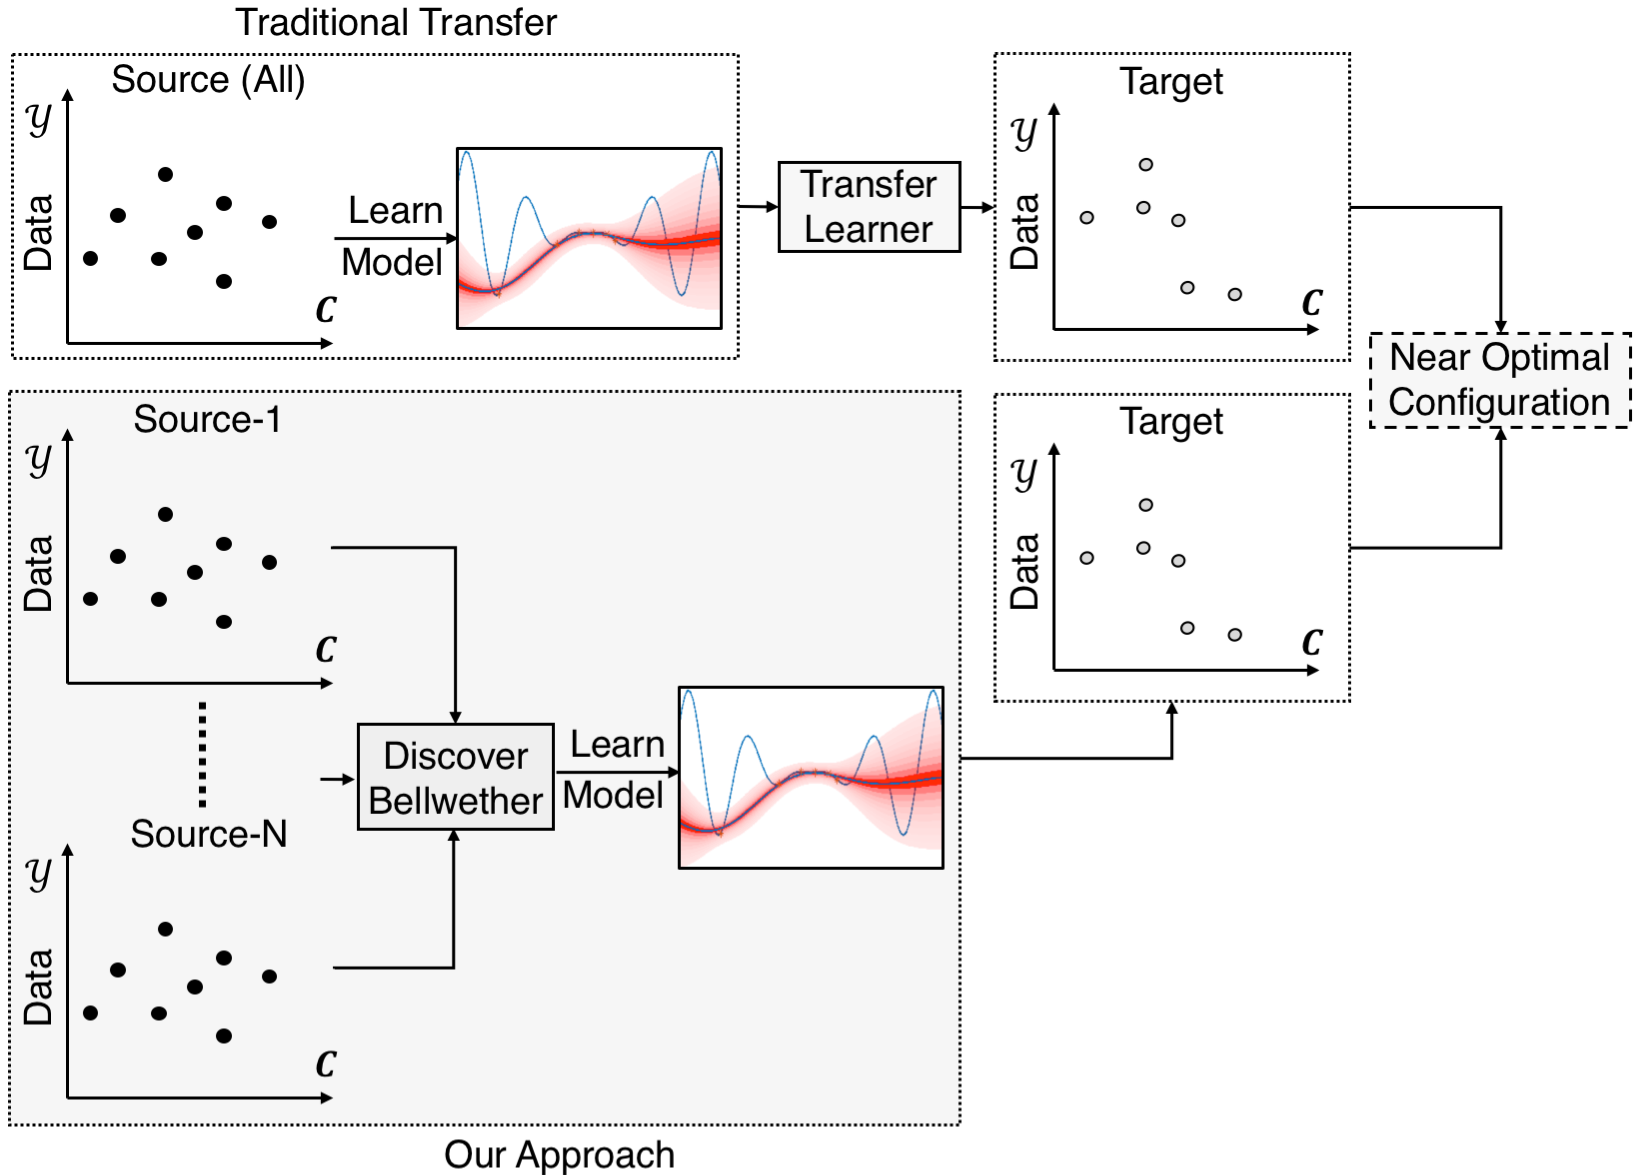
\includegraphics[width=\linewidth]{figures/compare.png}
    \caption{Traditional Transfer Learning compared with using bellwethers to 
    discover near optimal configurations.}
    \label{fig:intro_fig}
\end{figure}

Due to the shortcomings of  existing methods (expense), much recent work in  automatic
configuration~\cite{Nam2013, Nam2015, Jing2015, kocaguneli2011find,kocaguneli2012,turhan09,peters15, krishna18} has explored   {\em transfer learning}  for resolving `cold start' problems---problems starting anew for which collecting data is expensive.
Transfer learning typically entails the transfer of information from a selected
 software system operating in a ``\textit{source}'' environment to learn a  model for predicting the performance of the system in the 
``\textit{target}'' environment (i.e. a software system in a different environment).  

Prior work in the area of transfer learning focused on ``\textit{What to transfer}'' and ``\textit{How to transfer}'', by implicitly assuming that the source and target are related to each other. Hence, that work failed to address ``\textit{Where to transfer from}''~\cite{pan2010survey}. While studies have shown when transfer learning works, they do not offer methods for selecting a suitable source~\cite{jamshidi2017transfer2}.
Note that poor source selection can lead to {\em negative transfer}
i.e., we learn poor configurations from irrelevant prior knowledge. 

The issue of identifying a suitable source is a common problem in transfer learning. To address this, some researchers~\cite{krishna16,mensah17a, 
mensah17b, krishna18} have recently proposed the use of the \textit{bellwether} effect, which states that:
\begin{quote}
    ``When analyzing a community of software data, then within that community 
    there exists \underline{at least one} exemplary source, called 
    \underline{bellwether(s)}, which can best define predictors for other 
    datasets \ldots''
\end{quote}


The \textit{bellwether effect} has shown promise in identifying suitable 
sources for transfer learning in such varied domains as defect prediction, 
effort estimation, and code smell detection~\cite{krishna18}.
The significance of bellwethers is that they can be found very easily
(just a for-loop around wrapped around existing methods). Also, as shown in this paper and
others~\cite{krishna16,mensah17a,mensah17b, krishna18}, reasoning from the bellwether can lead to superior transfer (as compared to other transfer learning methods).

This paper is the first to attempt applying bellwethers to configuration problems. 
From a formal perspective, the BEETLE is similar to a  {\bf racing algorithm}
that sequentially evaluates candidates and discard poor ones as soon as statistically sufficient evidence is found (this elimination of inferior candidates leads to better conclusions~\cite{birattari2002racing}).
For more details on how BEETLE implements its racing algorithm, see \tion{beetle}.

This work  makes the  following research contributions: 
\begin{enumerate}[leftmargin=*]
\item \textit{Source selection}: We show that the \textit{bellwether effect} exists in performance optimization and that we can use this to discover suitable sources (called bellwether environments) to perform transfer learning. (\S\ref{subsec:rq1})
\item \textit{Fast source selection algorithm:} We develop a fast algorithm for discovering the bellwether environment by evaluating at-most $\approx10\%$ of the measured configuration space (\S\ref{sect:beetle}).
\item \textit{Transfer learning using Bellwethers:} We develop a novel transfer 
learning algorithm using bellwether called BEETLE (short for  
\underline{Be}llw\underline{e}ther \underline{T}ransfer \underline{Le}arner)
that uses the bellwether environment to construct a simple transfer learner 
(\S\ref{sect:beetle}).
\item \textit{More effective than non-transfer learning: } We show that using the BEETLE is just as good as than non-transfer learning approaches. It is also lot more economical. (\S\ref{sect:rq2}).
\item \textit{More effective than state-of-the-art methods: } Configurations discovered using the bellwether environment are better than the state-of-the-art 
methods~\cite{valov2017transferring, jamshidi2017transfer} (\S\ref{subsec:rq4}).

\item \textit{Reproduction Package: } To assist other researchers, a reproduction package with all our scripts and data are available online (see \url{http://tiny.cc/BEETLE}).
\end{enumerate}


\section{Definitions and Problem Statement}
\label{sect:formalization}
\noindent This  section offers definitions of concepts
 used in this paper. 
 
\noindent\textbf{Configuration: }A software system, $\mathcal{S}$, may offer a number of configuration options that can be changed. We denote the total number of configuration options of a software system $\mathcal{S}$  as $N$. A configuration option of the software system can either be a (1)~numeric value or a (2)~boolean flag. A configuration is represented by $c^{i}$, where $i$ represents the $i^{th}$ configuration of a system. A set of all configurations is called the \textit{configuration space}, denoted as $\mathcal{C}$.
  Formally, $\mathcal{C}$ is a Cartesian product of all possible options $\mathcal{C}$ = Dom($c_1$) $\times$ Dom($c_2$) $\times$ ... $\times$ Dom($c_N$), where $\text{Dom}(c_i) = \{0, 1\}$ (in our case) and $N$ is the number of configuration options. 

\begin{wrapfigure}{r}{1.8in}
    \scriptsize \centering
    \resizebox{1\linewidth}{!}{
\begin{tabular}{l|l|l|l|l }
                     & \texttt{-f} & \texttt{-i} & \texttt{-u} & \texttt{-v} \\\hline
$c^1$                & 0                            & 0                            & 0                            & 1                            \\\hline
$c^2$                & 0                            & 0                            & 1                            & 0                            \\\hline
\vdots & \vdots         & \vdots         & \vdots         & \vdots         \\\hline
$c^N$                & 1                            & 1                            & 1                            & 1                           
\end{tabular}}
    \caption{Some Unix  configuration options for  \texttt{mv}.}
    \label{fig:sample_config}
\end{wrapfigure}
As a simple example, consider the Unix move program \texttt{mv}, i.e., $\mathcal{S}\equiv\text{\texttt{mv}}$. The \texttt{mv} program offers four configuration options namely, -f (force move), -i    (interactive prompt), -u (update), and -v (verbose), ie., $N=4$. Sample configurations with these options are shown in \fig{sample_config}. %The configuration space $\mathcal{C}$ = Dom($c_1$) $\times$ Dom($c_2$) $\times$ Dom($c_3$) $\times$ Dom($c_N$).




\noindent\textbf{Environment: }
As defined by Jamshidi et al. \cite{jamshidi2017transfer2}, 
the different ways
a software system
is deployed and used is called its
  {\em environment} ($e$). 
The environment is usually defined in terms of: (1) \textbf{\textit{workload}} ($w$): the input of the system 
on which it operates on; (2) \textbf{\textit{hardware}} ($h$): the deployment configuration in 
which the system is running; and (3) \textbf{\textit{version}} ($v$): the state of the 
software. 
Note that, other environmental changes might be possible (e.g., JVM version used, etc.). For example, consider software system Apache Storm, here
we must ensure that an appropriate JVM is installed in an environment before it can be deployed in that environment. Indeed, the selection of one version of 
a JVM over another can have a profound performance impact. However, the perceived improvement in the performance is due to the optimizations in JVM, not the original software system being studied.  Therefore, in this paper, we do not alter the environment which does not have a direct impact on the performance of the software system. 

\noindent We use the following criteria to select the  environment:
\be[leftmargin=*]
    \item Environmental factors of the software systems that we can vary in the deployment stack of the system. This prevents us from varying factors such as JVM version, CPU frequency, system software, etc., which define the deployment stack and not the software system. 
    \item Common changes developers choose to alter in the software system. In practice, it is these factors that affect the performance of systems the most~\cite{jamshidi2017transfer2, jamshidi2017transfer, valov2017transferring, valov2015}. 
    \item Factors that are most amenable for transfer learning. Preliminary studies have shown that factors such as workload, hardware, and software version lend themselves very well to transfer learning~\cite{jamshidi2017transfer2, jamshidi2017transfer}.
\ee
For a more detailed description of the factors that were changed and those that were unchanged, see Table~\ref{tab:datasets}.

Formally, we say an environment is   $\mathit{\mathbf{e}}=\{w, h, v\}$ where $w \subseteq W$, $h \subseteq H$, and $v \subseteq V$. Here, $W, H, V$ are the space of all possible hardware changes $H$;   all possible software versions $V$, and all possible workload changes  $W$. With this, the environment space is defined as $\mathcal{E}\in\{W\times H\times V\}$, i.e., a subset of environmental conditions $\mathit{\mathbf{e}}$ for various workloads, hardware, and environments.

\noindent\textbf{Performance: } 
Each configuration ($c$) of a system $\mathcal{S}$ under an environment $\mathit{\mathbf{e}}$, 
has a corresponding performance measure $y \in Y_{S,c,e}$ associated with it. 
We denote the performance 
measure associated with a given configuration ($c^i$) by $y=f(c^i)$.  We 
consider the problem of finding the near-optimal configurations ($c^{*}$) such 
that $f(c^{*})$ is better (less/more) than other configurations in $C_{A,e}$. That is:
\begin{equation*}
\centering
     {\begin{array}{*{20}{l}}
     \centering
{f(c^{*}) \le f(c){\rm{~}}\forall c \in {C_{A,h,w,v}}\setminus c^{*} }&{{\text {for min objective}}}\\
{f(c^{*}) \ge f(c){\rm{~}}\forall c \in {C_{A,h,w,v}}\setminus c^{*} }&{{\text {for max objective}}}
\end{array}}
\end{equation*}

\noindent\textbf{Bellwethers: }
In the context of performance optimization, the bellwether  effect can be stated as following: \textit{For a configurable system, when performance measurements are made 
    under 
    different environments, then
     among those environments there exists one exemplary environment, called 
    the bellwether, which can be used determine near optimum configuration for 
    other environments for that system}.
We show that, when performing transfer 
learning, there are exemplar source environments called the bellwether 
environment(s) ($\mathcal{B}={e_{s1}, e_{s2},...,e_{sn}}\subset E$), which 
are the best source environment(s) to find near-optimal configuration for the 
rest of the environments ($\forall e \in E\setminus \mathcal{B}$). 


Using the above definitions, we now offer the following  \textbf{Problem Statement} 
for this paper:\\

 
\noindent\begin{minipage}{\linewidth}
    \begin{center}
    \arrayrulecolor{black}
    \begin{tabular}{|p{0.95\linewidth}|}
    \hline
         \rowcolor[HTML]{FFFFFF}
        Our goal is to find the near-optimal 
configuration for a target environment ($S_{e_t}$), by learning from the measurements ($\langle c,y\rangle$) for the same system operating in different source environments ($S_{e_s}$). 
\\\hline
    \end{tabular}
    \end{center}
\end{minipage}
\vspace{1mm} 

In other words, we aim to reuse the measurements from a system operating in an environment to optimize the same system operating in the different environment thereby reducing the number of measurements required to find the near-optimal configuration.
The rest of this paper describes and comparatively evaluates
different methods for achieving this goal (where one of those
methods is  BEETLE).


\section{{\large Beetle: Bellwether Transfer Learner}}
\label{sect:beetle}

\begin{figure}[t]
\centering
\begin{subfigure}[t]{\linewidth}
\centering
\textbf{Pick Bellwether Environment}\\[0.1cm]
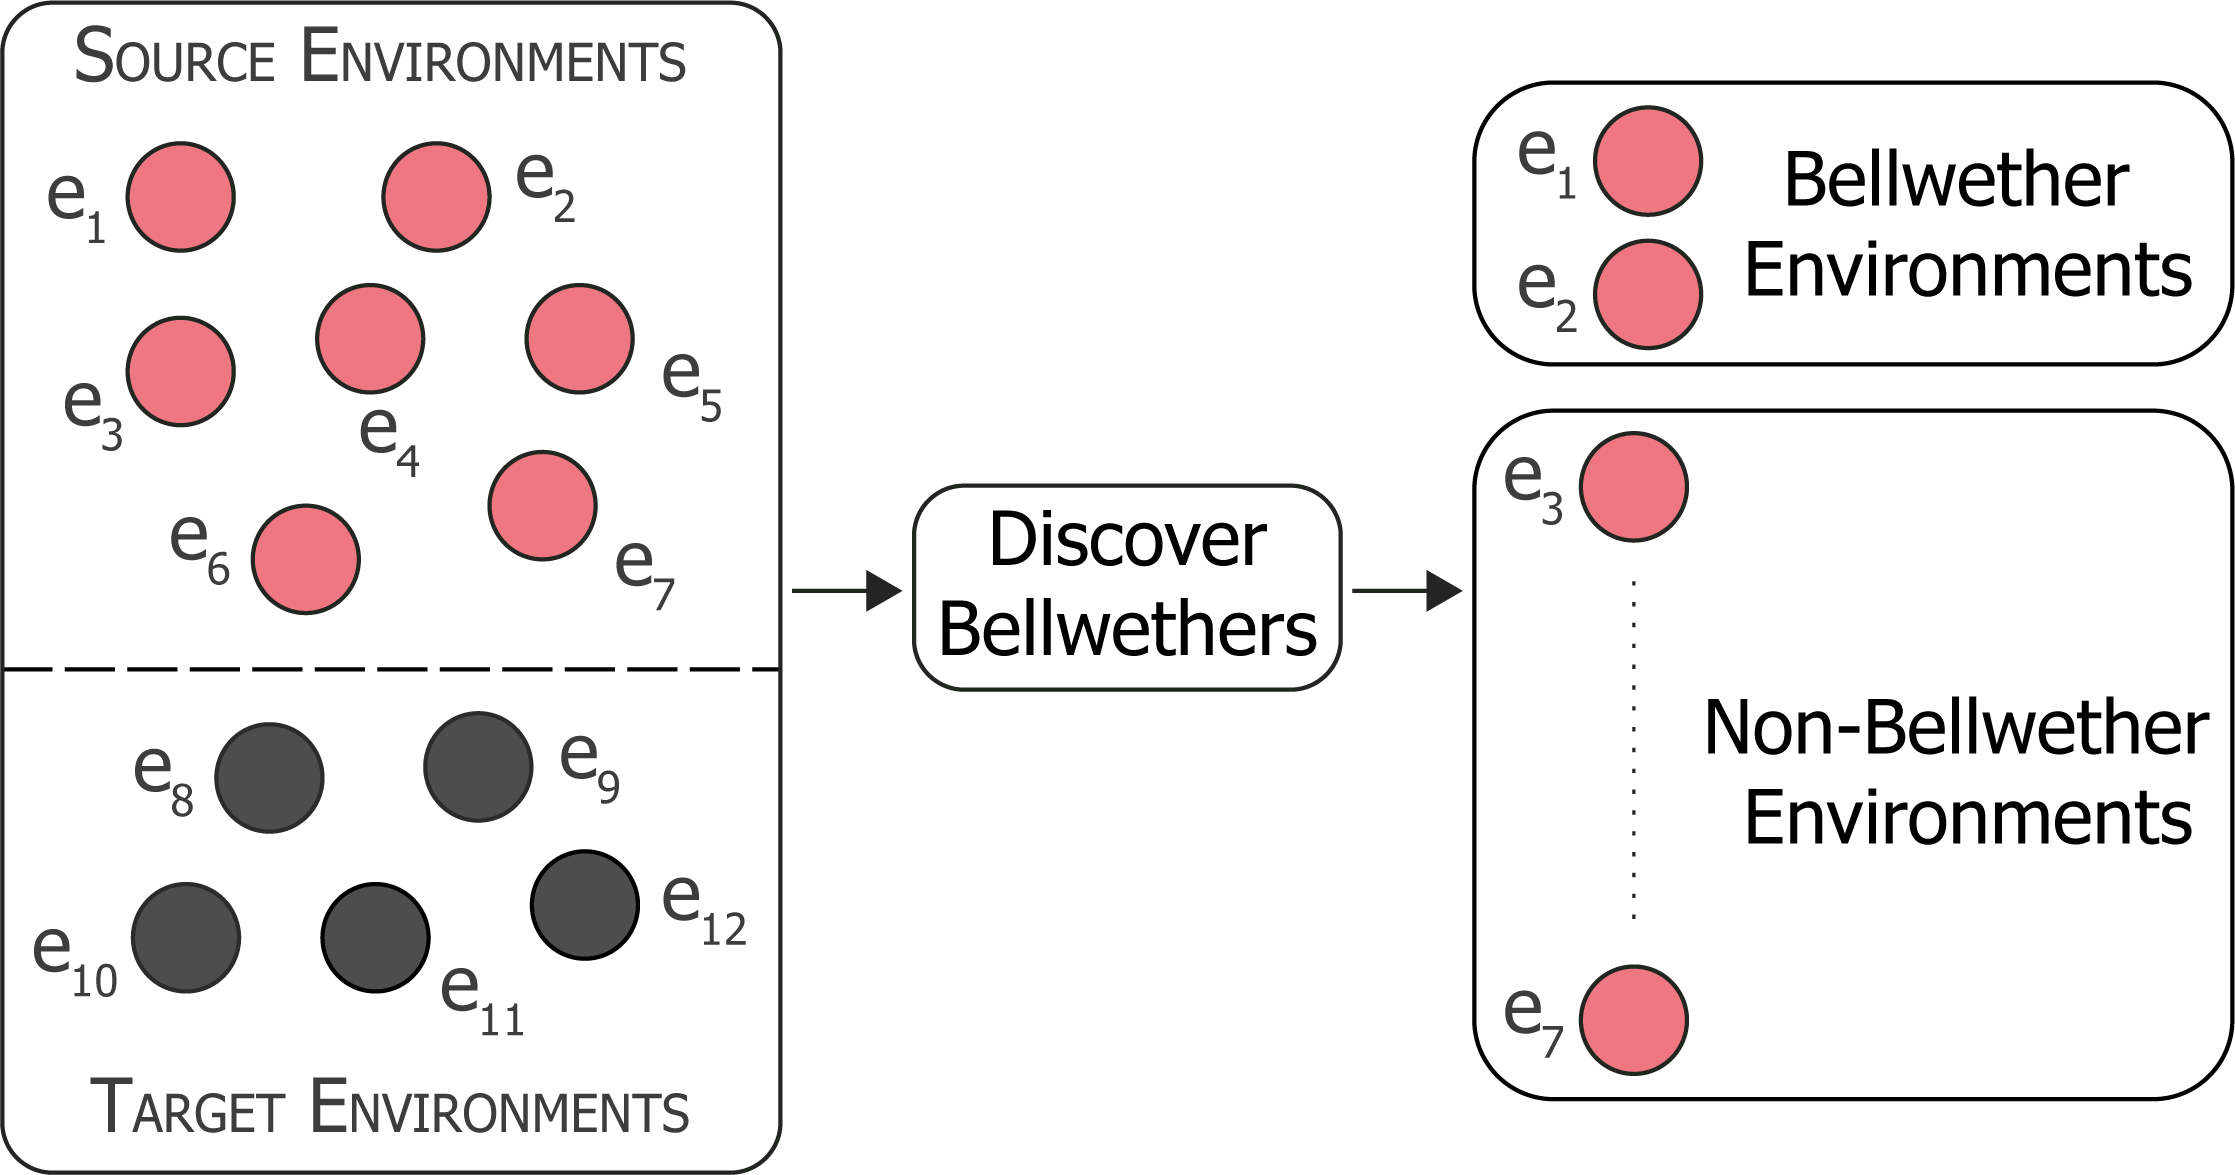
\includegraphics[width=\linewidth]{figures/source_target.png}
\end{subfigure}\\
\begin{subfigure}[t]{\linewidth}
\vspace{0.5cm}
\small
\begin{lstlisting}[xleftmargin=4.0ex,mathescape,frame=none,numbers=left]
def FindBellwether(sources, step_size, budget, thres, lives): 
  while lives or cost > budget:
   "Sample configurations"
   sampled = list()
   for source in sources:
     sampled += source.sample(step_size)
   "Get cost"
   cost = get_cost(sampled)
   "Evaluate pair-wise performances"
   perf = get_perf(sampled)
   "Remove non-bellwether environments"
   sources=remove_non_bellwethers(sources, perf, thres)
   "Loose life if no sources are removed"
   if prev == len(sources): lives -= 1
   "Return a bellwether"
  return sources[argmin(perf)]
\end{lstlisting}
\end{subfigure}
\caption{{\small This figure demonstrates how to pick the bellwethers}}
\label{fig:approach_a}
\end{figure}

\begin{figure}[t]
\begin{subfigure}[t]{\linewidth}
\centering
\textbf{Transfer Learning with Bellwether Environment}\\
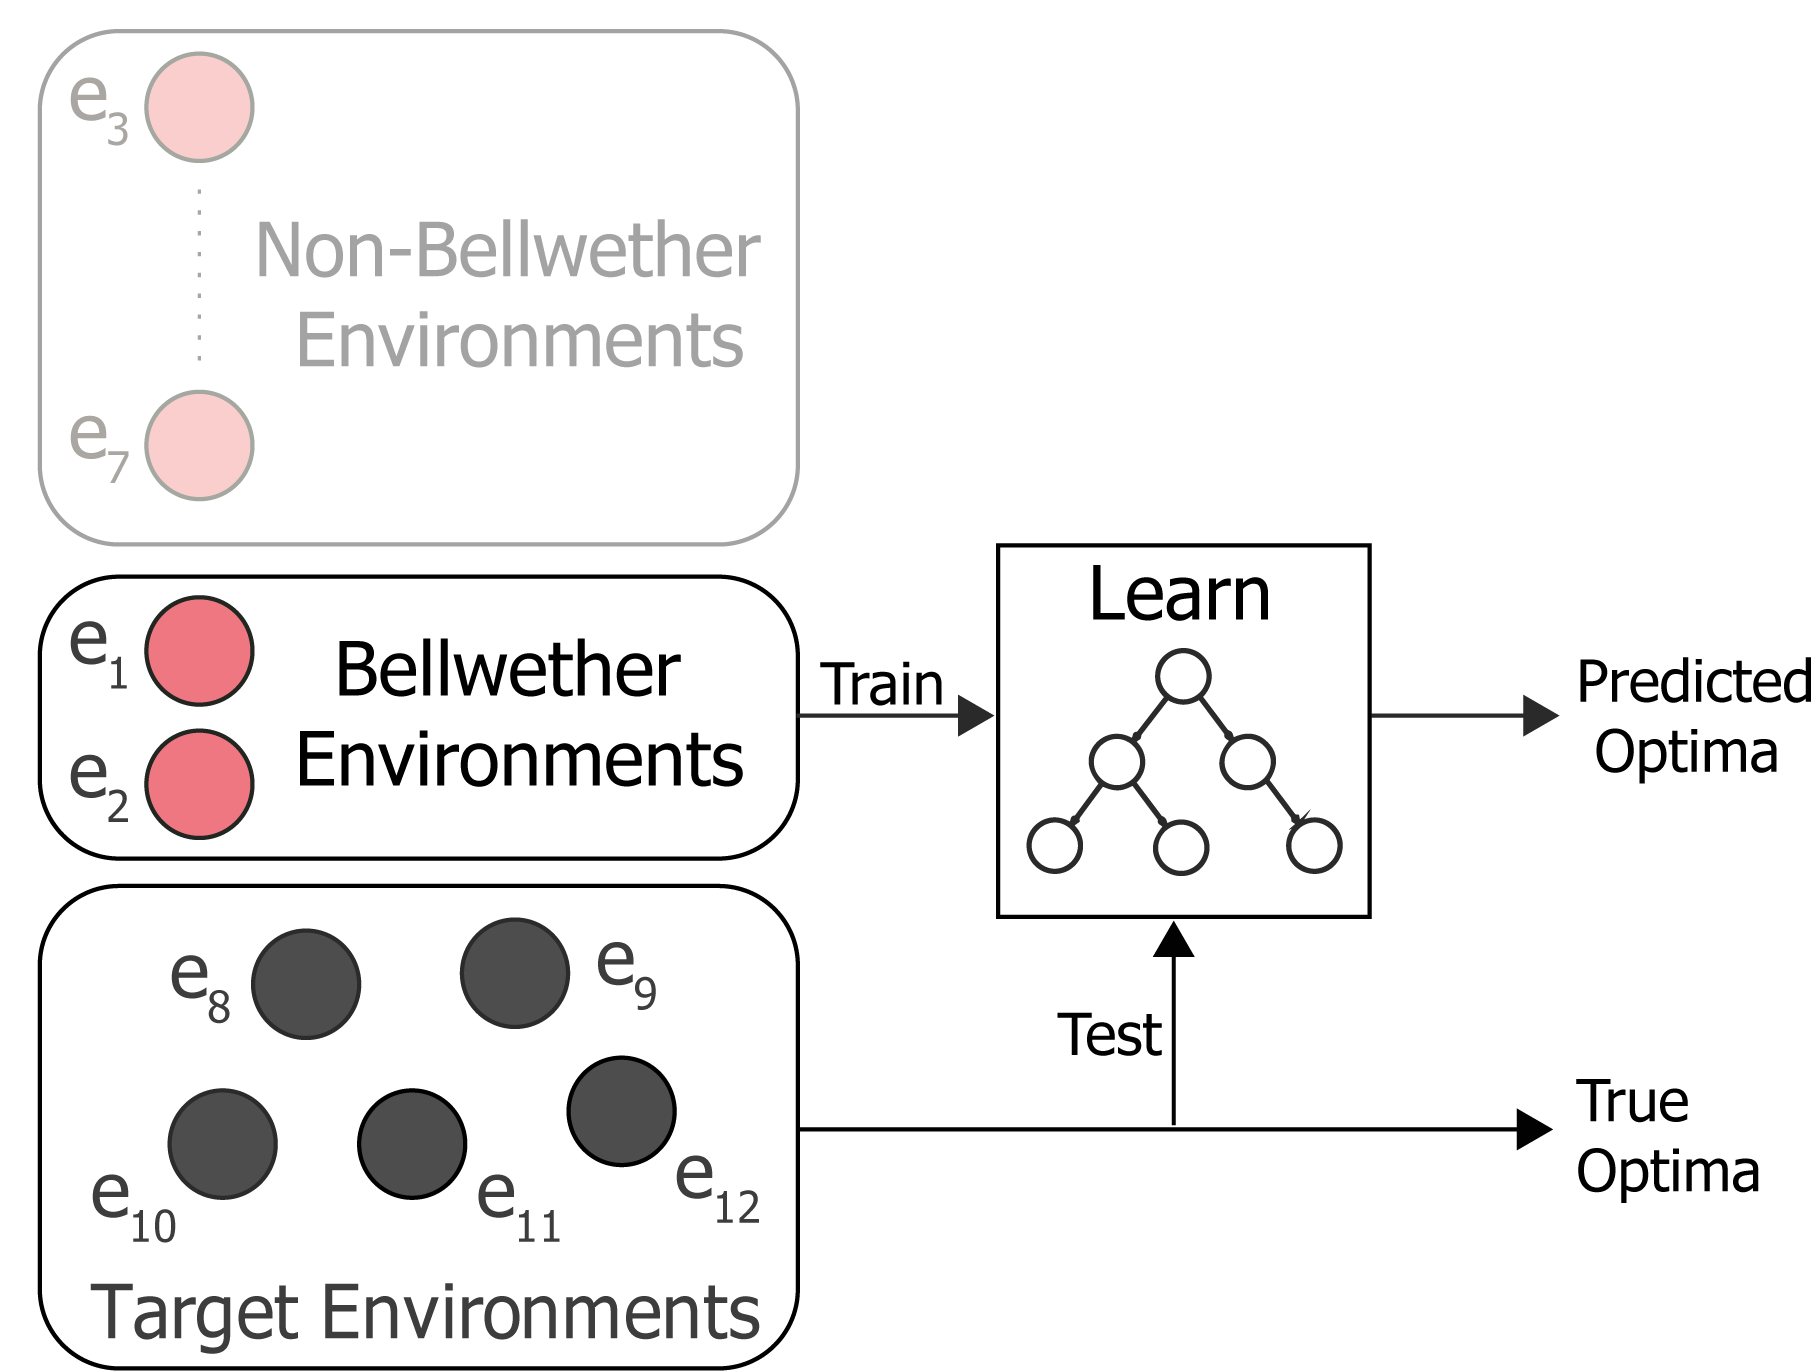
\includegraphics[width=0.85\linewidth]{figures/bellwether-transfer.png}
\end{subfigure}~~\\
\begin{subfigure}[t]{\linewidth}
\vspace{0.4cm}
\small
\begin{lstlisting}[xleftmargin=5.0ex,mathescape,frame=none,numbers=left]
def BEETLE(sources, target, budget): 
  "Find the bellwether environment"
  bellwether = FindBellwether(sources, step_size, budget, thres, lives)
  "Sample the bellwether source to fit budget"
  b_some = bellwether.sample(budget)
  "Train a prediction model with the bellwether"
  prediction_model = regTree.train(b_some)
  predicted = prediction_model.test(target.indep)
  return target[argmin(predicted)]
\end{lstlisting}
\end{subfigure}	
\caption{{\small This figure demonstrates how to construct BEETLE.}}
\label{fig:approach_b}
\end{figure}


% \begin{minipage}[]{0.475\linewidth}
% \begin{figure}
%     \centering
%     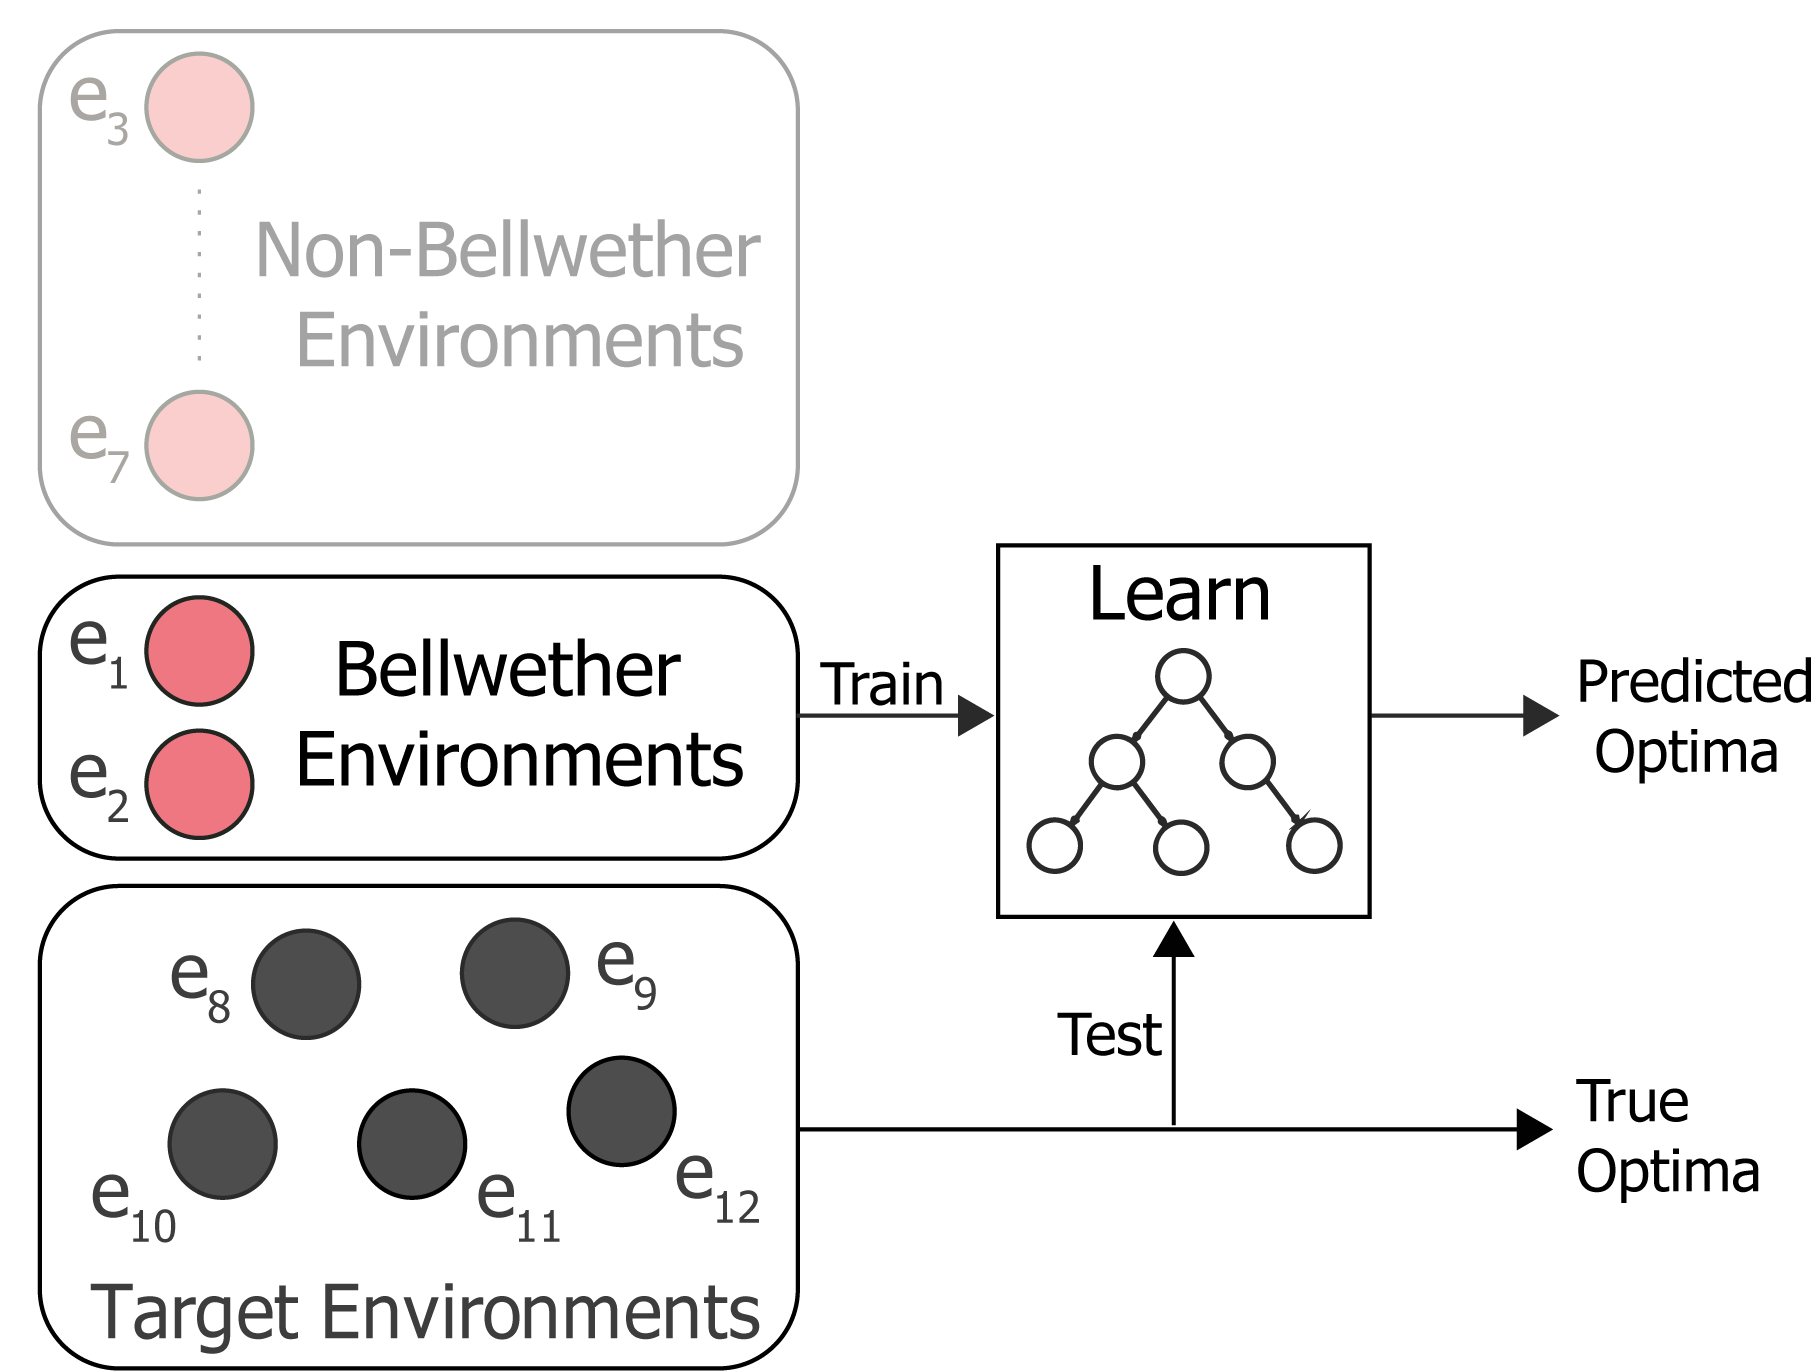
\includegraphics[width=\linewidth]{figures/bellwether-transfer.png}
% \end{figure}
% \end{minipage}\\
% \begin{minipage}[]{0.475\linewidth}

% \end{minipage}
% \begin{minipage}[]{0.475\linewidth}
% \begin{figure}[t]
% \small
% \hspace{0.2cm}\begin{lstlisting}[xleftmargin=5.0ex,mathescape,frame=none,numbers=left]
% def FindExemplar(sources, step_size, budget, lives=4): 
%   # Initializing Data Structures
%   all = model = perf = dict()
%   prev = len(sources)
%   while True:
%     # Sample new configurations and its corresponding
%     # performance measures
%     for source in sources: 
%      all[source].indep = source.sample(step_size)
%      all[source].dep = get_perf(all[source].indep)
%     for source in sources:
%      # Train a model of each source using the
%      # sampled configurations
%      model[source]=regTree()
%      model[source]=train(all[source].indep,
%                                    all[source].dep)
%      # For all the other datasets, find the performance 
%      # NAR of the model
%      for target in sources:
%       if source != target:
%          perf[source][target] = 
%               get_pairwise_perf(all[source],all[target])
%     # Find the statistics of the performance of all models
%     mean, std = get_stats(perf)
%     # Remove all the source, which performance 
%     # worse than (mean + 1*std)
%     sources = remove_not_promising(perf, (mean + std))
%     # If no sources are removed, loose life
%     if prev == len(sources): lives -= 1
%     # If total number of measurements exceed the budget, exit
%     if count(all) > budget or lives == 0: break
%   # Return the source which has the lowest performance delta 
%   return min(perf)
% \end{lstlisting}
% \end{figure}
% \end{minipage}


This section describes BEETLE, a bellwether based-approach that finds the near-optimal configuration using the knowledge in the bellwether environment. BEETLE can be separated into the following main steps: (i) finding the bellwether environment, and (ii) using the bellwether environment to find the near-optimal configuration for target environments. That is, BEETLE has then two key components:
\be
    \item \textit{Identifying the bellwether environment:} To train a transfer model, we use the bellwether effect to discover the best source environments (known as the \textit{bellwether environment}) among the available environments. 
    
    \item \textit{Construct the Transfer Model:} Next, to perform transfer learning, we use these bellwether environments to train a performance prediction model with \textbf{regression tree}~\cite{breiman1996bagging}.
\ee

Our intuition is that if a bellwether source environment is carefully selected, then it is possible to build a simple transfer model without any complex methods and still be able to generate near-optimal configurations in a target environment. 

In Figures~\ref{fig:approach_a} \&~\ref{fig:approach_b}, we describe BEETLE and list an algorithm of BEETLE. In this example, there are seven source environments ($e_1, e_2,..., e_7$), which have been optimized previously. $e_8, e_9,..., e_{12}$ represents the target environments, which need to be optimized. BEETLE\textquotesingle s objective is to find a bellwether among the source environments and use it to find the near-optimal configuration for the target environments. 

\subsection{Finding Bellwether Environments}\label{subsec:finding}

From a formal perspective of finding a bellwether, BEETLE     is a  {\bf racing algorithm} that sequentially evaluates candidates and discards poor ones as soon as statistically sufficient evidence is found. The premise of such racing
algorithms are that the elimination of inferior candidates speeds up the procedure and allows to evaluate promising candidates on more instances to obtain more reliable estimates of their behavior~\cite{birattari2002racing}.

Fig.~\ref{fig:approach_a} shows how we find  bellwethers. The process starts by randomly sampling a small subset of configurations from the source environments. The size of the subset (of configurations) is controlled by a predefined parameter \textit{step\_size}, which defines the number of configurations to be sampled in each iteration (Line 6). 

The cost of sampling the configuration is calculated (Line 8). In our case, we use the number of measurements as a proxy for cost. But, this can be replaced by any user-defined cost function (\textit{get\_cost}). To compute the effectiveness of an environment, the sampling configurations along with the performance measure is used to build a performance model (regression tree in this case). Please note that we chose regression tree as a model because it has been extensively used for performance prediction of configurable
software systems and provided good results~\cite{guo2013variability, sarkar2015cost, nair2017faster, nair2017using, nair2018finding, guo2017data, valov2017transferring}. 

Then, this model is used to predict the optimal configuration among the configurations sampled in Line 7 (Line 11). We only used the sampled configurations because the actual performance of a source can only be calculated if the actual performance values (associated with the configurations) are known. This process is repeated for all the environments (represented as \textit{sources}) under consideration. Depending on how an environment can find the near-optimal configuration for other environments and a user-defined threshold (\textit{thres}), non-bellwether environments are eliminated (Line 12). Non-bellwether environments are environments, which are not able to find near-optimal configurations for the other environments.  If the no environment is eliminated (with more
data) when compared to the previous iteration
(lesser data), then a life is lost (Line 14). When all lives are
expired or we run out of the budget, the search process terminates. The environment with maximum performance is returned as the bellwether (Line 16). Please note that, \textit{FindBellwether} can identify multiple bellwethers ($e_1, e_2$). Also, note that the motivation behind using the parameter lives is to detect
convergence of the search process and avoid resource wastage.



\vspace{-0.2cm}
\subsection{Using Bellwethers}

Once the bellwether environment is identified, it can be used to find the near-optimal configurations of target environments. As shown in Fig.~\ref{fig:approach_b},   \textit{FindBellwether} returns the predicted bellwether environment (Line 3). Performance modeling then samples the bellwether environments (Line 5) for some number of samples (a user-defined parameter called budget).
Please note that a user might choose to reuse the measurement used in \textit{FindBellwether} and save on cost. The sampled configurations and their corresponding performance measures are used to build a prediction model (Line 7). Similar to \textit{FindBellwether}, we use a regression tree as our modeling method of choice. The prediction model is then used to predict the optimal configuration in the for the target environment (Lines 8-9). The predicted optimal configuration is returned as the best configuration. This process is then repeated for each target environments ($e_8, e_9,..., e_{12}$).



\vspace{-0.1cm}
\section{Transfer Learning in Performance Optimization}
\label{sect:tl}

This section described the systems we use to evaluate  BEETLE comparatively.
These alternate systems are   (a)~two state-of-the-art transfer learners for performance optimization: Valov et al.~\cite{van2017automatic} and Jamshidi et al.~\cite{jamshidi2017transfer}; and (b) a non-transfer learner: Nair et al.~\cite{nair2017using}. For details on these systems, see below.

\begin{table*}[t]
\caption{{\small Overview of the real-world subject systems. $|C|$:Number of Configurations, $|c|$=Number of configuration options, $|E|$: Number of Environments, $|H|$: Hardware, $|W|$: Workloads, and $|V|$: Versions. See \protect\url{http://tiny.cc/bw_software} for more details.}}
\label{tab:datasets}
\scriptsize
\resizebox{\textwidth}{!}{%
\begin{tabular}{@{}lp{1cm}p{1.6cm}p{2cm}p{2.3cm}p{0.5cm}p{1.2cm}p{3.5cm}@{}}
\toprule
\textbf{System} & \textbf{Language} & \textbf{\{$|C|$, $N$, $|E|$\}} & \multicolumn{1}{c}{\textbf{$H$}} & \multicolumn{1}{c}{\textbf{$W$}} & \multicolumn{1}{c}{\textbf{$V$}} & \multicolumn{1}{c}{\textbf{Unchanged}} & \textbf{Description} \\ \midrule

\rowcolor[HTML]{EFEFEF}
x264 & C, Assembly & 4000, 16, 21 & NUC/4/1.30/15/SSD NUC/2/2.13/7/SSD Station/2/2.8/3/SCSI, AWS/1/2.4/1.0/SSD, AWS/1/2.4/0.5/SSD, Azure/1/2.4/3/SCSI & 8/2, 32/11, 128/44 & r2389, r2744 & Memory, CPU, background services & {\sc x264} is a video encoder that compresses video files and has 16 configurations options to adjust output quality, encoder types, and encoding heuristics. \\
SPEAR & C, Assembly & 16384, 14, 10 & NUC/4/1.30/15/SSD, NUC/2/2.13/7/SSD, Station/2/2.8/3/SCSI, AWS/1/2.4/1.0/SSD, AWS/1/2.4/0.5/SSD, Azure/1/2.4/3/SCSI & (in \#variables
 /\#clauses), 774/5934, 1008/7728,, 1554/11914, 978/7498 & 1.2, 2.7 & Memory, CPU, background services & {\sc Spear} is an industrial strength bit-vector arithmetic decision procedure and Boolean satisfiability (SAT) solver. It is designed for proving software verification conditions, and it is used for bug hunting. \\
\rowcolor[HTML]{EFEFEF}
SQLite & C & 1000, 14, 15 & NUC/4/1.30/15/SSD, NUC/2/2.13/7/SSD, Station/2/2.8/3/SCSI, AWS/1/2.4/1.0/SSD, AWS/1/2.4/0.5/SSD, Azure/1/2.4/3/SCSI & write--seq, read--batch, , read--rand, read--seq & 3.7. 6.3, 3.19.0.0 & Memory, CPU, background services & {\sc SQLite} is a lightweight relational database management system, embedded in several browsers and operating systems, which has 14 configuration options to change indexing and features for size compression.\\
SaC & C & 846, 50, 7 & NUC/4/1.30/15/SSD, NUC/2/2.13/7/SSD, Station/2/2.8/3/SCSI, AWS/1/2.4/1.0/SSD, AWS/1/2.4/0.5/SSD, Azure/1/2.4/3/SCSI & random matrix generator,, particle filtering, differential, equation solver, k-means, , optimal matching, nbody , simulation, conjugate , gradient, garbage collector. & 1.0.0 & Memory, CPU, background services & {\sc SaC} is a compiler for high-performance computing. The SaC compiler implements a large number of high-level and low-level optimizations to tune programs for efficient parallel executions. \\
\rowcolor[HTML]{EFEFEF}
Storm & Clojure & 2048, 12, 4 & NUC/4/1.30/15/SSD, NUC/2/2.13/7/SSD, Station/2/2.8/3/SCSI, AWS/1/2.4/1.0/SSD, AWS/1/2.4/0.5/SSD, Azure/1/2.4/3/SCSI & WordCount, RollingCount, RollingSort, SOL & Storm 0.9.5 + Zookeeper 3.4.11 & JVM machine, Zookeeper Options, Memory, CPU, background services & {\sc Storm} is a distributed stream processing framework which is used for data analytics. We run three benchmarks and measure the latency of the benchmarks. \\ 
\bottomrule
\end{tabular}
}

\end{table*}
\vspace{-0.2cm}
\subsection{Transfer Learning with Linear Regression}

Valov et al.~\cite{valov2017transferring} proposed an approach for transferring performance models of software systems across platforms with \textit{different hardware settings}. The method consists of the following two components: 
\bi
\item \textit{Performance prediction model:} The configuration source hardware are sampled using \textit{Sobol} sampling. The number of configurations is given by $T\times N_f$, where $T={3, 4, 5}$ is the \textit{training coefficient} and $N_f$ is the number of configuration options. These configurations are used to construct a \textit{Regression Tree} model.
\item \textit{Transfer Model:} To transfer the predictions from the source to the target, a linear regression model is used since it was found to provide good approximations of the transfer function. To construct this model, a small number of random configurations are obtained from the source and the target. 
\ei

\vspace{-0.2cm}
\subsection{Transfer Learning with Gaussian Process} 


Jamshidi et al.~\cite{jamshidi2017transfer} took a slightly different approach to transfer learning. They used Gaussian Processes (GP) to find the relatedness between the performance measures in source and the target. The relationships between input configurations were
captured in the GP model using a covariance matrix that
defined the kernel function to construct the Gaussian processes model. To encode the relationships between the measured performance of the source and the target, a scaling factor is used with the above kernel. 

% \begin{figure}[t]
\small
\begin{lstlisting}[xrightmargin=6ex, mathescape,frame=none,numbers=right]
def LinearTransform(source, target, 
                    training_coef, budget): 
  "Construct a prediction model"
  prediction_model=regTree.train(source, training_coef)
  "Sample random measurements"
  s_samp = source.sample(budget)
  t_samp = target.sample(budget)
  "Get performance measurements"
  s_perf=get_perf(s_samp)
  t_perf=get_perf(t_samp)
  "Train a transfer model with LR"
  transfer_model=linear_model.train(s_perf, t_perf)
  return prediction_model, transfer_model
\end{lstlisting}
\caption{\small{Linear Transformation Transfer. From Valov et al.~\cite{valov2017transferring}.}}
\label{fig:lineartransform}  
\end{figure}
% \begin{figure}[t]
\small
\begin{lstlisting}[xrightmargin=6ex, mathescape,frame=none,numbers=right]
def GPTransform(source, target, 
                 source_budget, target_budget): 
  "Sample random configurations"
  s_some = source.sample(source_budget)
  t_some = target.sample(target_budget)
  "Get performance measurements"
  s_perf = get_perf(s_some)
  t_perf=get_perf(t_some)
  "Compute correlation"
  perf_correlation = get_correlation(s_perf, t_perf)
  "Compute covariance"
  input_covariance = get_covariance(s_some, t_some)
  "Construct a kernel"
  kernel = input_covariance $\times$ perf_correlation
  "Train the Gaussian Process model"
  learner = GaussianProcessRegressor(kernel)
  prediction_model = learner.train(s_some)
  return prediction_model
\end{lstlisting}
\caption{\small{Gaussian Process Transformation Transfer. From   Jamshidi et al.~\cite{jamshidi2017transfer}.}}
\label{fig:gptransform}  
\end{figure}



The new kernel function is a defined as follows:
\begin{equation}
    k(s, t, f(s), f(t)) = k_t(s, t) \times k_{xx}(f(s), f(t)),
\end{equation}\label{eq:gpkernel}
where $k_t(s,t)$ represents the multiplicative scaling factor. $k_t(s,t)$ is given by the correlation between source f(s) and target f(t) function, while $k_{xx}$ is the covariance function for input environments (s \& t). The essence of this method is that the kernel captures the interdependence  between the source and target environments. 
\vspace{-0.2cm}
\subsection{Non-Transfer Performance Optimization}
\label{sect:nair}
A performance optimization model with no transfer was proposed by Nair et al.~\cite{nair2017using} in FSE '17. It works as follows: 
\be[leftmargin=*]
\item Sample a small set of measurements of configurations from the target environment.
\item Construct performance model with regression trees. 
\item Predict for near-optimal configurations. 
\ee
The key distinction here is that unlike transfer learners, that use a \textit{different source environment} to build to predict for near-optimal configurations in a target environment, a non-transfer method such as this uses configurations \textit{from within the target} environment to predict for near-optimal configurations. 

\section{Experimental Setup}
\label{sect:expt}
\subsection{Subject Systems}
\label{sect:datasets}
In this study, we selected five real-world configurable software systems from different domains, with different functionalities (a video encoder, an SAT solver, the SQLite database, a high-performance C-compiler, and streaming data analytics tool), written in different programming languages, and of varying sizes (Spear contains 16384 measurements). We selected these software systems since their characteristics cover a broad spectrum of scenarios with different size of the configuration space. \tab{datasets} lists the details of the software systems used here.

\subsection{Evaluation Criterion}
\label{sect:eval}
Typically, performance models are evaluated based on the accuracy or error using measures such as MMRE. 
 MMRE is defined as:
\[
    MMRE = \frac{|predicted-actual|}{actual} \cdot 100
\]
Recently, it has been shown that exact measures like MMRE
can be somewhat misleading for the purposes of assessing
configurations.
In fact, there have been a lot of criticism regarding MMRE. MMRE along with other accuracy statistics such as MBRE have been shown to cause conclusion instability~\cite{myrtveit2012validity, myrtveit2005reliability, foss2003simulation}.

Nair et al.~\cite{nair2017using} showed that even when exact MMRE values may be erroneous, the {\em relative rankings} of the  performance scores are still useful . Especially for pruning away less-than-desirable
configurations~\cite{nair2017using}.    

\begin{figure*}[t]
{\small
    \begin{minipage}[]{0.475\linewidth}
    \textbf{{\sc X264}}\\
    \resizebox{\linewidth}{!}{%
    \arrayrulecolor{lightgray}%
    \begin{tabular}{|llrrc|}
    \arrayrulecolor{lightgray}
    \rowcolor{lightgray}{\small \textbf{Rank}} & {\small\textbf{Dataset}} & {\small \textbf{Median}} & {\small\textbf{IQR}} & \\\hline  
    \rowcolor{lightergray}  1 &      x264\_18 &    0.35  &  1.82 & \quart{0}{2}{0}{1} \\
    \rowcolor{lightergray}  1 &       x264\_9 &    0.35  &  1.62 & \quart{0}{2}{0}{1} \\
    \hline  2 &      x264\_10 &    0.94  &  8.25 & \quart{0}{12}{1}{1} \\
      2 &       x264\_7 &    0.94  &  8.25 & \quart{0}{12}{1}{1} \\
      2 &      x264\_11 &    1.62  &  7.46 & \quart{1}{11}{2}{1} \\
    %   2 &       x264\_1 &    1.62  &  7.46 & \quart{1}{11}{2}{1} \\
    %   2 &       x264\_8 &    1.62  &  7.46 & \quart{1}{11}{2}{1} \\
     3 &      x264\_16 &    2.33  &  12.18 & \quart{0}{18}{3}{1} \\
      3 &       x264\_2 &    2.33  &  12.18 & \quart{0}{18}{3}{1} \\
    %   3 &       x264\_5 &    2.33  &  12.18 & \quart{0}{18}{3}{1} \\
    %   3 &       x264\_4 &    2.33  &  12.18 & \quart{0}{18}{3}{1} \\
    3 &       x264\_6 &    2.82  &  5.35 & \quart{0}{8}{4}{1} \\  
    3 &      x264\_20 &    3.65  &  13.74 & \quart{1}{20}{5}{1} \\
      4 &      x264\_19 &    6.95  &  41.97 & \quart{3}{62}{10}{1} \\
      4 &       x264\_3 &    8.68  &  49.78 & \quart{6}{73}{12}{1} \\
        4 &      x264\_17 &    13.61  &  32.32 & \quart{5}{48}{20}{1} \\
      4 &      x264\_13 &    16.42  &  51.65 & \quart{2}{76}{24}{1} \\
      4 &      x264\_15 &    20.14  &  50.68 & \quart{4}{75}{29}{1} \\
    %   4 &      x264\_12 &    20.14  &  50.68 & \quart{4}{75}{29}{1} \\
      5 &      x264\_14 &    27.24  &  42.74 & \quart{3}{63}{40}{1} \\
      5 &       x264\_0 &    28.63  &  49.77 & \quart{6}{73}{42}{1} \\
    \hline \end{tabular}}\\
    \textbf{{\sc Sac}}\\
    \resizebox{\linewidth}{!}{%
    \begin{tabular}{|llrrc|}
    \arrayrulecolor{lightgray}
    \rowcolor{lightgray}{\small \textbf{Rank}} & {\small\textbf{Dataset}} & {\small \textbf{Median}} & {\small\textbf{IQR}} & \\\hline
    \rowcolor{lightergray}  1 &        sac\_6 &    0.27  &  0.14 & \quart{0}{0}{0}{0} \\
    \hline  2 &        sac\_4 &    0.96  &  4.26 & \quart{0}{3}{0}{0} \\
    %   2 &        sac\_7 &    0.97  &  4.04 & \quart{0}{3}{0}{0} \\
      2 &        sac\_8 &    1.04  &  3.67 & \quart{0}{3}{0}{0} \\
      2 &        sac\_9 &    2.29  &  4.98 & \quart{1}{4}{1}{0} \\
      3 &        sac\_5 &    10.8  &  89.65 & \quart{8}{71}{8}{0} \\
    \hline \end{tabular}}\\
    \textbf{{\small {\sc Storm} }}\\
    \resizebox{\linewidth}{!}{%
    \begin{tabular}{|llrrc|}
    \arrayrulecolor{lightgray}
    \rowcolor{lightgray}{\small \textbf{Rank}} & {\small\textbf{Dataset}} & {\small \textbf{Median}} & {\small\textbf{IQR}} & \\\hline  
    \rowcolor{lightergray}  1 & storm\_feature9 &    0.0  &  0.0 & \quart{0}{0}{0}{1999} \\
    \rowcolor{lightergray}  1 & storm\_feature8 &    0.0  &  0.0 & \quart{0}{0}{0}{1999} \\
    \rowcolor{lightergray}  1 & storm\_feature6 &    0.0  &  0.01 & \quart{0}{19}{0}{1999} \\
    \rowcolor{lightergray}  1 & storm\_feature7 &    0.01  &  0.04 & \quart{0}{79}{19}{1999} \\
    \hline \end{tabular}}
    \end{minipage}\hspace{10pt}
    \begin{minipage}[]{0.475\linewidth}
    \textbf{{\small {\sc Spear}}}\\[0.1cm]
    \resizebox{\linewidth}{!}{%
    \begin{tabular}{|llrrc|}
    \arrayrulecolor{lightgray}
    \rowcolor{lightgray}{\small \textbf{Rank}} & {\small\textbf{Dataset}} & {\small \textbf{Median}} & {\small\textbf{IQR}} & \\\hline  
    \rowcolor{lightergray} 1 &      spear\_7 &    0.1  &  0.1 & \quart{0}{1}{1}{13} \\
    \rowcolor{lightergray}  1 &      spear\_6 &    0.1  &  0.2 & \quart{0}{2}{1}{13} \\
    \rowcolor{lightergray}  1 &      spear\_1 &    0.1  &  0.1 & \quart{0}{1}{1}{13} \\
    \rowcolor{lightergray}  1 &      spear\_9 &    0.1  &  0.5 & \quart{0}{6}{1}{13} \\
    \rowcolor{lightergray}  1 &      spear\_8 &    0.1  &  0.2 & \quart{0}{2}{1}{13} \\
    \rowcolor{lightergray}  1 &      spear\_0 &    0.1  &  0.91 & \quart{0}{12}{1}{13} \\
    \hline  2 &      spear\_5 &    0.28  &  0.3 & \quart{2}{4}{3}{13} \\
      3 &      spear\_4 &    0.6  &  1.17 & \quart{5}{16}{8}{13} \\
      4 &      spear\_2 &    1.09  &  5.31 & \quart{8}{71}{14}{13} \\
      5 &      spear\_3 &    1.89  &  4.48 & \quart{18}{61}{25}{13} \\
    \hline \end{tabular}}\\[0.2cm]
    \textbf{{\small {\sc Sqlite}}}\\[0.1cm]
    \resizebox{\linewidth}{!}{%
    \begin{tabular}{|llrrc|}
    \arrayrulecolor{lightgray}
    \rowcolor{lightgray}{\small \textbf{Rank}} & {\small\textbf{Dataset}} & {\small \textbf{Median}} & {\small\textbf{IQR}} & \\\hline  
    \rowcolor{lightergray}  1 &    sqlite\_17 &    0.8  &  1.13 & \quart{0}{1}{0}{0} \\
    \rowcolor{lightergray}  1 &    sqlite\_59 &    2.0  &  3.44 & \quart{0}{4}{2}{0} \\
    \rowcolor{lightergray}  1 &    sqlite\_19 &    2.0  &  4.88 & \quart{0}{6}{2}{0} \\
    \hline  2 &    sqlite\_44 &    1.96  &  6.91 & \quart{0}{10}{2}{0} \\
      2 &    sqlite\_16 &    2.52  &  7.41 & \quart{1}{10}{3}{0} \\
      2 &    sqlite\_73 &    2.82  &  7.24 & \quart{1}{10}{3}{0} \\
      2 &    sqlite\_45 &    3.47  &  11.86 & \quart{0}{17}{4}{0} \\
      2 &    sqlite\_10 &    3.88  &  6.92 & \quart{1}{9}{4}{0} \\
      2 &    sqlite\_96 &    4.94  &  6.04 & \quart{1}{8}{6}{0} \\
      2 &    sqlite\_79 &    5.64  &  5.24 & \quart{4}{7}{7}{0} \\
      2 &    sqlite\_11 &    6.64  &  5.75 & \quart{5}{8}{8}{0} \\
      2 &    sqlite\_52 &    6.84  &  7.95 & \quart{1}{11}{8}{0} \\
      2 &    sqlite\_97 &    7.68  &  13.71 & \quart{7}{18}{10}{0} \\
      3 &    sqlite\_18 &    13.17  &  54.68 & \quart{5}{74}{17}{0} \\
      3 &    sqlite\_94 &    27.43  &  47.66 & \quart{9}{65}{37}{0} \\
    \hline \end{tabular}}
    % \textbf{{\small STORM 1}}\\[0.1cm]
    % \resizebox{\linewidth}{!}{ 
    % \begin{tabular}{|llrrc|}
    % \arrayrulecolor{lightgray}
    % \rowcolor{lightgray}{\small \textbf{Rank}} & {\small\textbf{Dataset}} & {\small \textbf{Median}} & {\small\textbf{IQR}} & \\\hline  
    % 1 & storm1\_feature8 &    2.27  &  7.34 & \quart{0}{11}{3}{1} \\
    % \hline  2 & storm1\_feature7 &    12.13  &  27.98 & \quart{0}{41}{18}{1} \\
    % \hline  3 & storm1\_feature6 &    16.03  &  35.5 & \quart{5}{53}{23}{1} \\
    % \hline  4 & storm1\_feature9 &    50.88  &  29.77 & \quart{35}{44}{75}{1} \\
    % \hline \end{tabular}}
    \end{minipage}
    \caption{ {\small Median NAR of 30 repeats. Median NAR is the normalized absolute residual values  as described in Equation~\ref{eq:nar}, and IQR the difference between 75th percentile and 25th percentile found during multiple repeats. Lines with a dot in the middle (~\protect\quartex{-2}{13}{6}), show the median as a round dot within the IQR. All the results are sorted by the median NAR: a lower median value is better. The left-hand column (\textit{Rank}) ranks the various techniques where lower ranks are better.}}
    \label{fig:rq1}
}
\end{figure*}
For this reason, Nair et al.~\cite{nair2017using} argued for the use alternatives to MMRE in the performance optimization. Specifically, they propose \textit{rank-based metrics}. Here, the accuracy of a model is measured  by sorting the values of $y=f(x)$ from `small' to `large', that is:
\begin{equation}
    f(c_1) \le f(c_2) \le f(c_3) \le ... \le f(c_n).
\end{equation}

\noindent The predicted rank is then compared to the actual rank to compute the differences in ranking. We note that rank difference, though effective, is not particularly informative since it is sensitive to the workload. This means that in some workloads, \textit{a small difference in performance measure can lead to a large rank difference and vice-versa}. For example, in {\sc Spear\_0} the top performance of the optimal configuration (rank 1) and 100$^{th}$ best configuration has a difference of 0.09\%---which means a large rank difference of 100 does not mean poor performance. 

Hence, we define a performance measure called \textit{Normalized Absolute Residual} (NAR), which represents the normalized difference between the actual performance measurements of the optimal configuration and the predicted optimal configuration. It is defined as: 
\begin{equation}
\label{eq:nar}
{ \tiny
    \mathit{NAR} = \frac{min(f(c)) - f(c^{*})}{max(f(c)) - min(f(c))} \cdot 100
}
\end{equation}
where $c \in C_{A,h,w,v} \setminus c^*$. This measure is equivalent to Absolute Residual (lower is better). However, in our setting the range of the performance measures across different environments are not equal (hence the need for a normalization step). Formally, NAR is a variant of of Generational Distance or Inverted Generation Distance which used in search-based software engineering~\cite{wang2016practical, chen2018sampling, deb2002fast}.

\subsection{Statistical Validation}
\label{sect:stats}

Our experiments are all subjected to inherent randomness introduced by sampling configurations or by different source and target environments. To overcome this, we use 30 repeated runs, each time with a different random number seed. The repeated runs provide us with a sufficiently large sample size for statistical comparisons. Each repeated run collects the values of NAR to assess the the transfer learners.

To rank these 30 numbers collected as above, we use the Scott-Knott test 
recommended by Mittas and Angelis~\cite{mittas13}. The Scott-Knott test has been endorsed by several SE researchers~\cite{leech2002call, poulding10, arcuri11, shepperd12a, kampenes07, Kocaguneli2013:ep}. Scott-Knott is a non-parametric statistical test that performs a bootstrap test with 95\% confidence~\cite{efron93} to determine the existence of statistically significant differences. This followed by an A12 test to check that any observed differences were not trivially small effects~\cite{Vargha00}. We say that a ``small'' effect has $a <0.6$. 
Scott-Knott test results in treatments being ranked from best to worst. Note, statistically similar treatments will have the same ranks.

\section{Results}
\label{sect:results}

\noindent Our results are structured as answers to the following research questions.

\subsection*{RQ1: Does there exist a Bellwether Environment?}\label{subsec:rq1}

\noindent\textbf{\textit{\underline{Purpose:}}} The first research question seeks to establish the presence of  bellwether environments within different environments of a software system.\\
\textbf{\textit{\underline{Approach:}}} For each subject software system, we use the environments to perform a pair-wise comparison as follows:
\be[leftmargin=*]
\item We pick one environment as a source and evaluate all configurations to construct a transfer learner.
\item The remaining environments is used as targets. For every target environment, we use the transfer learner constructed in the previous step to predict for the best configuration.
\item Then, we measure the NAR of the predictions (see \tion{eval}). % Briefly, this NAR reports the normalized absolute difference between predicted optima and the true optima of these target environments.
\item Afterwards, we repeat steps 1, 2, and 3 for all the other source environments and gather the outcomes.
\item Finally, we use Scott-Knott test to rank each environment (and its usefulness as a source).
\ee
\textbf{\textit{\underline{Result:}}}
Our results are shown in Fig.~\ref{fig:rq1}. Overall, we find that there is always at least one environment (the bellwether environment) in all the subject systems, that is much superior to others. Note that, {\sc Storm} is an interesting case, here all the environments are ranked 1, which means that all the environments are equally useful as a bellwether environment
---in such cases any randomly selected environment could serve as a bellwether. 
Further, we note that the variance in the bellwether environments are much lower compared to other environments. 
% Please note, in our experiments (except for SPEAR); we only use a sample of the configuration space to claim the existence of Bellwether. To further understand the implications of sampling, we redid the same experiment without 20\% of the configuration to assert if the bellwether is dependent on how we sampled the original configuration space (which is infeasible to measure). We found that the bellwether environment remains the same. We do not present the result due to space restrictions. 

Since  sampling does not influence our results, we can say:
\vskip 1ex
\noindent\begin{minipage}{\linewidth}
    \begin{center}
    \arrayrulecolor{black}
    \begin{tabular}{|p{0.95\linewidth}|}
    \hline
         \rowcolor[HTML]{EFEFEF} \textbf{\textit{\underline{Summary}}} There exists environments in each subject system, which act as the bellwether environment and hence can be used to find the near-optimal configuration for the rest of the environments.\\\hline
    \end{tabular}
    \end{center}
    \end{minipage}
    \vspace{0.1cm}

\begin{table}[t]
{\small
    \centering
    \caption{{\small Effectiveness of source selection method.}}
    \label{tbl:method}
    \begin{tabular}{@{}ccccc@{}}
    \toprule
    \multirow{2}{*}{\textbf{Subject System}} & \multicolumn{2}{c}{\textbf{\begin{tabular}[c]{@{}c@{}}Bellwether\\ Environment\end{tabular}}} & \multicolumn{2}{c}{\textbf{\begin{tabular}[c]{@{}c@{}}Predicted Bellwether\\ Environment\end{tabular}}} \\ \cmidrule(l){2-5} 
     & \textbf{Median} & \textbf{IQR} & \textbf{Median} & \textbf{IQR} \\ \midrule
    SQLite & 0.8 & 1.13 & 1.8 & 2.48 \\
    Spear & 0.1 & 0.1 & 0.1 & 0 \\
    x264 & 0.35 & 1.62 & 0.9 & 1.06 \\
    Storm & 0.0 & 0.0 & 0.0 & 0.0 \\
    SaC & 0.27 & 0.14 & 0.63 & 7.4 \\ \bottomrule
    \end{tabular}
}
\end{table}



\vspace{-0.25cm}
\subsection*{RQ2: How many measurements are required to discover bellwether environments?}



\noindent\textbf{\textit{\underline{Purpose:}}} The bellwether environments found in RQ1 required us to use 100\% of the measured performance values from all the environments\footnote{Note, except for SPEAR, we only have measured a subset of all possible configuration space since we were limited by the time and the cost required to make exhaustive measurements}. Sampling all configurations may not be practical, since that may take an extremely long time~\cite{jamshidi2017transfer2}. %It can be prohibitively expensive to run and test all configurations of subject systems since their configuration spaces are large. 
Thus, in this research question, we ask if we can find the bellwether environments sooner using fewer samples. \\
\textbf{\textit{\underline{Approach:}}}
We used the racing algorithm discussed in Section~\ref{subsec:finding}. To see if our proposed method is effective, we compare the performance of bellwether environment with the predicted bellwether environment.

% It works as follows
% \be
% \item We start from 1\% of configurations from each environment and assume that every environment is a potential bellwether environment.
% \item Then, we increment the number of configurations in steps of 1\% and measure the NAR values. 
% \item We rank the environments and eliminate those that do not show much promise. A detailed description of how this is accomplished can be found in~\S\ref{sect:beetle}. 
% \item We repeat the above steps until we cannot eliminate any more environments.
% \ee
% The above strategy uses $\mu+\sigma$ of the NAR values at each step as a threshold to eliminate non-bellwether environments. To function correctly, this requires the NAR values to follow a normal distribution. If normality is violated, we used power transforms to make the data more normal distribution-like. We note that this is a common strategy commonly used in other domains to reduce the size of options or alternatives~\cite{borgelt2005keeping} and is also known as \textit{backward elimination}~\cite{blum1997selection}.
\begin{figure*}[t]
	\centering
\begin{subfigure}[t]{0.33\linewidth}
		\centering
		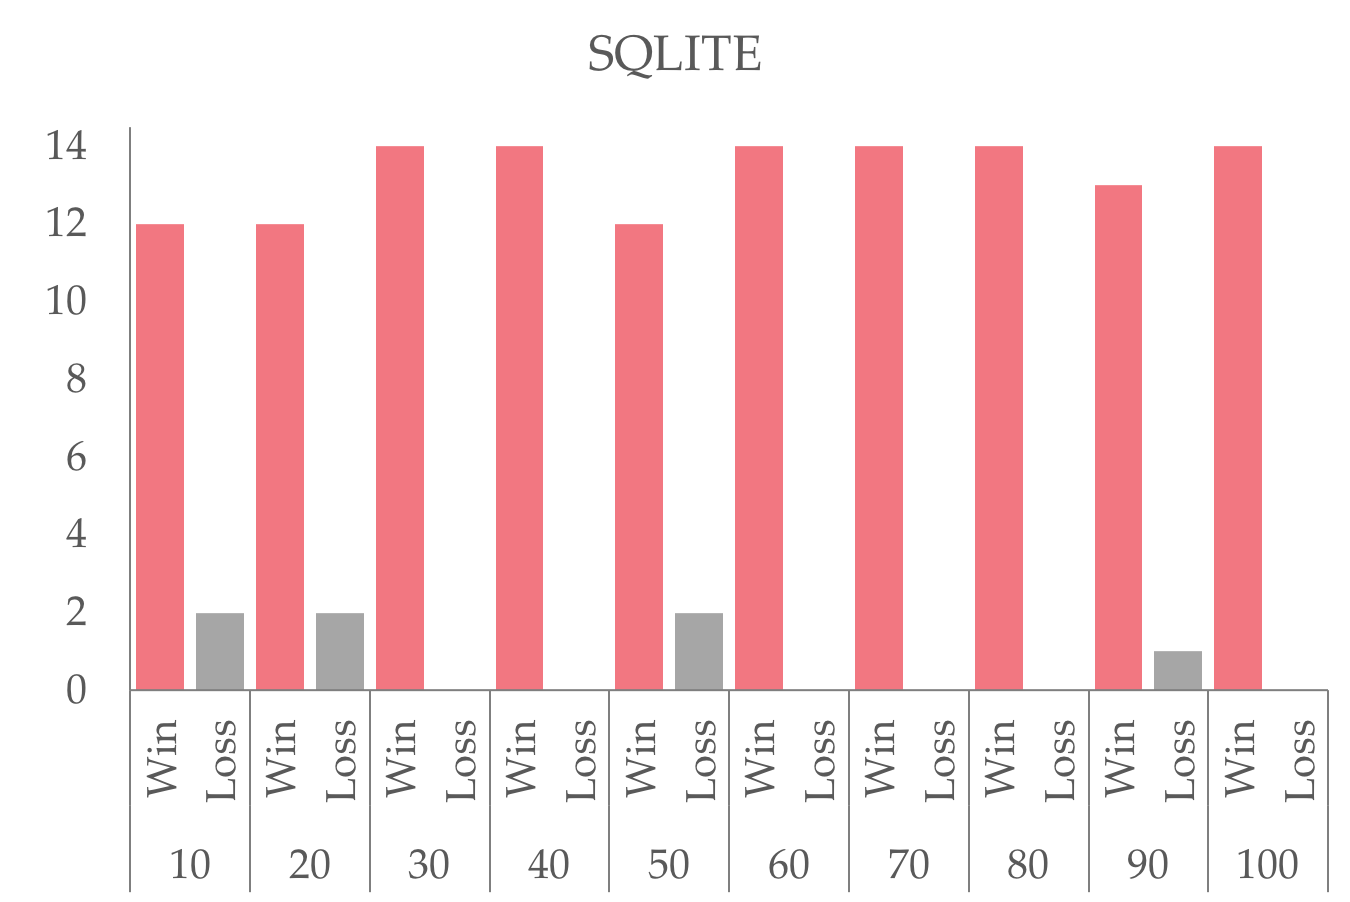
\includegraphics[width=\linewidth]{figures/sqlite_rq2.png}
\end{subfigure}%
\begin{subfigure}[t]{0.33\linewidth}
		\centering
		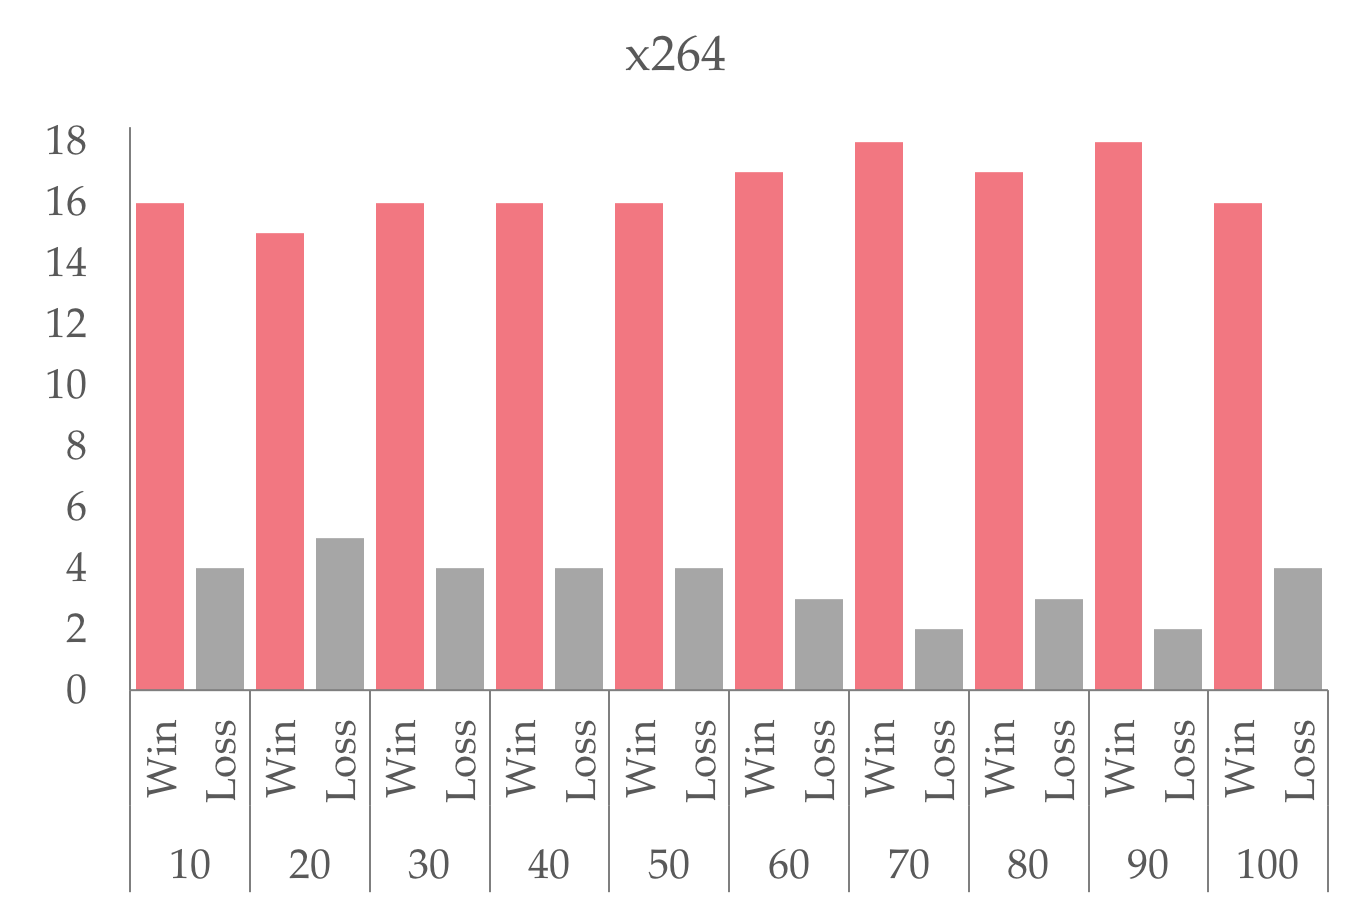
\includegraphics[width=\linewidth]{figures/x264_rq2.png}
\end{subfigure}%
\begin{subfigure}[t]{0.33\linewidth}
		\centering
		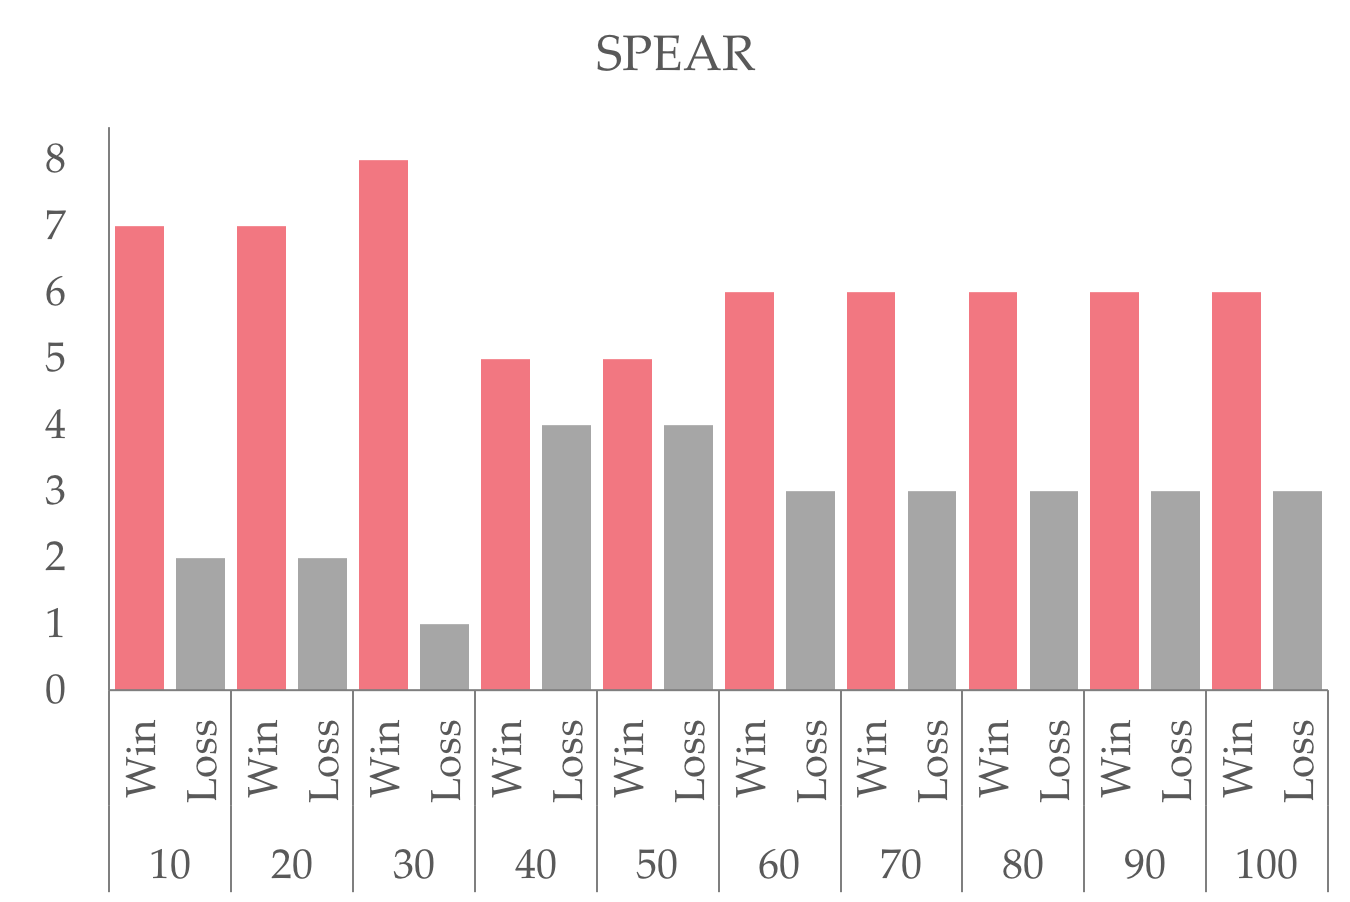
\includegraphics[width=\linewidth]{figures/spear_rq2.png}
\end{subfigure}\\[0.25cm]
\begin{subfigure}[t]{0.33\linewidth}
		\centering
		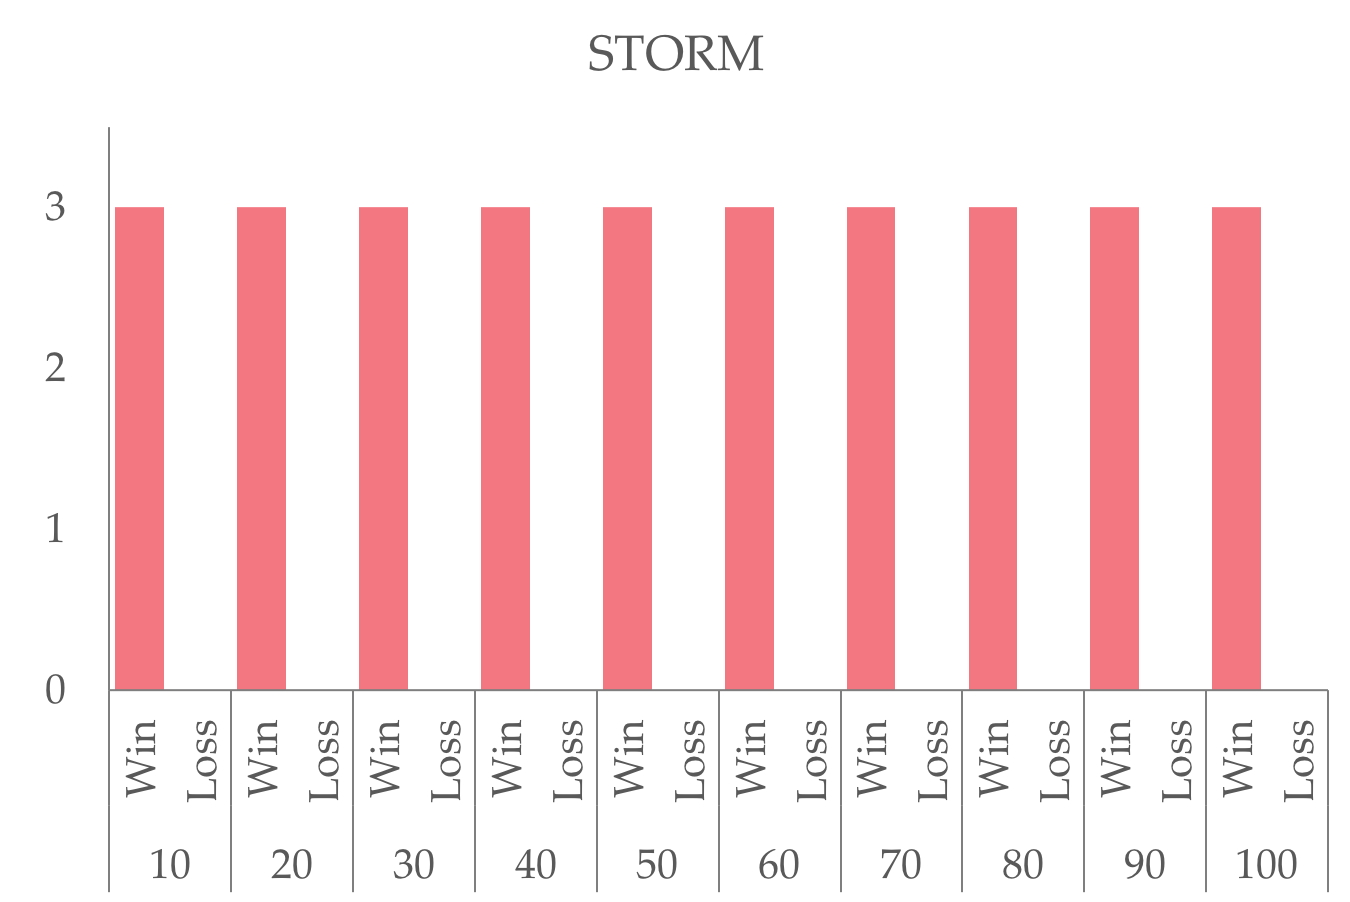
\includegraphics[width=\linewidth]{figures/storm_rq2.png}
\end{subfigure}\hspace{12pt}
\begin{subfigure}[t]{0.33\linewidth}
		\centering
		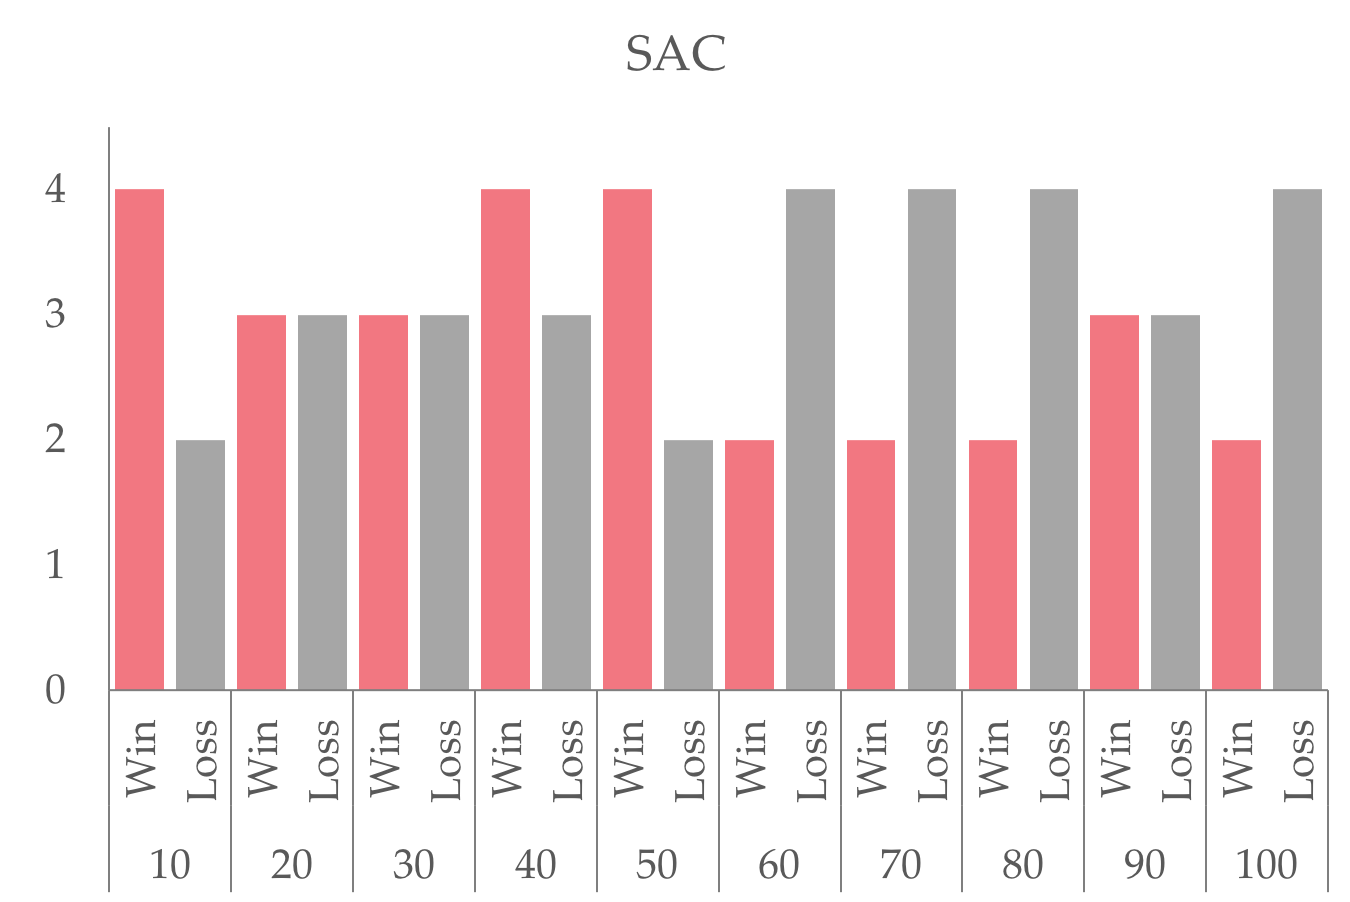
\includegraphics[width=\linewidth]{figures/sac_rq2.png}
\end{subfigure}\\[0.25cm]
	\caption{{\small Win/Loss analysis of learning from the bellwether environment and target environment using Scott Knott. The x-axis represents the percentage of data used to build a model and y-axis is the count.
	BEETLE wins in all models except for SAC-- and there only there when we have measured 50+\% of the data.}}
	\label{fig:rq2_1}
\end{figure*}

\noindent\textbf{\textit{\underline{Result:}}}
Table~\ref{tbl:method} summarizes our findings. We find that, 
\begin{itemize}[leftmargin=*]
    \item In all 5 cases, using at most 10\% of the configurations we find one of the bellwether environments that are found with 100\% of the measured configurations. See, column Rank in Table~\ref{tbl:method}. 
    \item In terms of quality of predictions, the NAR of the predicted bellwether environments with 10\% of the configurations is different by $<1\%$ from the bellwether found at 100\%.
\end{itemize}

 \begin{figure}[!t]
    \centering
    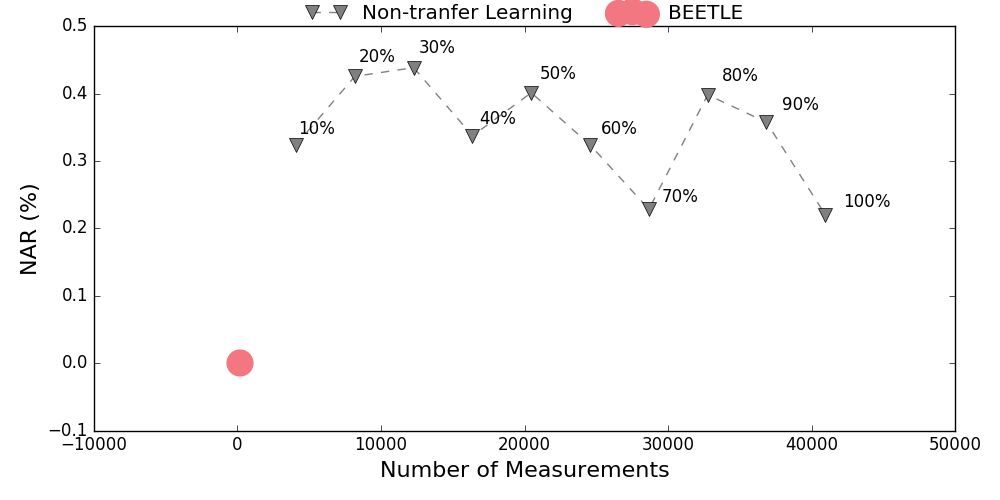
\includegraphics[width=1.04\linewidth]{figures/x264.png}
    \caption{{\small Trade-off between the quality of the configurations and the cost to build the model for {\sc x264}. The cost to find a good configuration using bellwethers is much lower than that of non-transfer-learning methods. }}
    \label{fig:tradeoffx264}
\end{figure}
These  results are most encouraging:

%One may argue that this answer to this question trivially could be answered as "yes" since one could not expect all environments to exhibit identical performance, there will always be some environment that can make better predictions. However, observe that the environments ranked first performs much better than the rest (with certain exceptions), and hence, the difference between the bellwether environment and others is not coincidental.


 \vskip 1ex
\noindent\begin{minipage}{\linewidth}
    \begin{center}
    \arrayrulecolor{black}
    \begin{tabular}{|p{0.95\linewidth}|}
    \hline
         \rowcolor[HTML]{EFEFEF} \textbf{\textit{\underline{Summary}}} The bellwether environment can be recognized using only a fraction of the measurements (under 10\%). Encouragingly, the identified bellwether environments have similar NAR values to the actual bellwether environment.  Note the importance of this results: running fewer configuration takes less time and is cheaper.\\\hline
    \end{tabular}
    \end{center}
    \end{minipage}
    \vspace{0.1cm}
 

%  Note the importance of this results: running fewer configuration takes less time to collect and is cheaper (e.g. measured in cloud CPU time).
%  Hence, we  can assert that discovering bellwether environments is economically very useful.
 
 
\vspace{-0.1cm}
\subsection*{RQ3: How does BEETLE compare to non-transfer  methods?}
\label{sect:rq2}

\noindent\textbf{\textit{\underline{Motivation}}}: We explore how BEETLE  compares to a non-transfer learning approach. For our experiment, we use the non-transfer performance optimizer proposed by Nair et al.~\cite{nair2017using}.
Both BEETLE and Nair et al.'s methods seek to achieve the same goal---find the optimal configuration in a target environment. BEETLE uses configurations from a \textit{different source} to achieve this, whereas the non-transfer learner uses configurations from \textit{within the target}. Please note BEETLE only uses 10\% of the configurations from the bellwether environment.\\
\textbf{\textit{\underline{Approach:}}} Our setup involves evaluating the Win/Loss ratio of BEETLE to the non-transfer learning algorithm while predicting for the optimal configuration. Comparing against true optima, we define ``win'' as cases where BEETLE has a better (or same) optima as the non-transfer learner or a ``loss''.\\
\textbf{\textit{\underline{Result:}}}
Our results are shown in Figures~\ref{fig:rq2_1} and \ref{fig:tradeoffx264}. In \fig{rq2_1}, the x-axis represents the number of configurations (expressed in \%) to train the non-transfer learner and BEETLE, and the y-axis represents the number of wins/losses. We observe:
\begin{itemize}[leftmargin=*]
\item \textit{Better performance:} In $\frac{4}{5}$ systems, BEETLE ``wins'' significantly more than it ``losses''. This means that BEETLE is better than (or similar to) non-transfer learning methods. 
\item \textit{Lower cost:} In terms of cost, we note that BEETLE outperforms the non-transfer learner significantly, ``winning'' at configurations of 10\%  to 100\% of the original sample size. Further, when we look at the trade-off between performance and number of measurements in \fig{tradeoffx264}, we note that BEETLE achieves a NAR close to zero with around 100 samples. Also, the non-transfer learning method of Nair et al.~\cite{nair2017using} has significantly larger NAR while also requiring large sample sizes. Hence, we say:\\
\end{itemize}
\vskip 1ex
\noindent\begin{minipage}{\linewidth}
    \begin{center}
    \arrayrulecolor{black}
    \begin{tabular}{|p{0.95\linewidth}|}
    \hline
     \rowcolor[HTML]{EFEFEF} \textbf{\textit{\underline{Summary}}} BEETLE performs better than (or same as) a non-transfer learning approach. BEETLE is also cost/time efficient as it requires far fewer measurements.\\\hline
    \end{tabular}
    \end{center}
    \end{minipage}
    \vspace{0.1cm}
\vspace{-0.1cm}
\subsection*{RQ4: How does BEETLE compare to state-of-the-art methods?}\label{subsec:rq4}

\noindent\textbf{\textit{\underline{Purpose:}}} The main motivation of this work is to show that the source environment can have a significant impact on transfer learning.  In this research question, we seek to compare BEETLE with other state-of-the-art transfer learners by Jamshidi et al.~\cite{jamshidi2017transfer} and Valov et al.~\cite{valov2017transferring}.\\
\textbf{\textit{\underline{Approach:}}} We perform transfer learning the methods proposed by Valov et al.~\cite{valov2017transferring} and Jamshidi et al.~\cite{jamshidi2017transfer} (see~\tion{tl}). Then we measure the NAR values and compare them statistically using Skott-Knott tests. Finally, we rank the methods from best to worst based on their Skott-Knott ranks.\\
\textbf{\textit{\underline{Result:}}}
Our results are shown in Fig.~\ref{fig:rq4}. In this figure, the best transfer learner is ranked 1. We note that in 4 out of 5 cases, the baseline transfer learner based on source selection performs just as well as (or better than) the state-of-the-art. This result is encouraging in that it points to significant impact choosing a good source environment can have on the performance of transfer learners. Further, in ~\fig{rq4_measurement} we compare the number of performance measurements required to construct the transfer learners (note the logarithmic scale on the vertical axis). Based on these results, we say:
%results, BEETLE requires far fewer measurements compared to the other transfer-learning methods. %Considering the scalability and negative transfer issues (as discussed in Section 1) of the state of the art techniques along with the effectiveness of BEETLE using (much) fewer configurations, we recommend using BEETLE.

\vskip 1ex
\noindent\begin{minipage}{\linewidth}
    \begin{center}
    \arrayrulecolor{black}
    \begin{tabular}{|p{0.95\linewidth}|}
    \hline
         \rowcolor[HTML]{EFEFEF} \textbf{\textit{\underline{Summary}}} In most software systems, BEETLE performs just as well as (or better than) other state-of-the-art transfer learners for performance optimization using far fewer measurements.\\\hline
    \end{tabular}
    \end{center}
    \end{minipage}
    \vspace{0.1cm}

\begin{figure}[htbp!]
{\scriptsize
    \begin{minipage}[]{\linewidth}
    \textbf{{\sc Sac}}\\[0.05cm] 
    \resizebox{\linewidth}{!}{% 
    \begin{tabular}{|llrrc|}
    \arrayrulecolor{lightgray}
    \rowcolor{lightgray}{\small \textbf{Rank}} & {\small\textbf{Learner}} & {\small \textbf{Median}} & {\small\textbf{IQR}} & \\\hline  
    \rowcolor{lightergray}  1 &       Jamshidi et al.~\cite{jamshidi2017transfer} &    1.58  &  5.39 & \quart{0}{4}{0}{0} \\\hline
      2 &     BEETLE &    6.89  &  99.1 & \quart{0}{79}{5}{0} \\
      2 &     Valov et al.~\cite{valov2017transferring} &    6.99  &  99.24 & \quart{0}{79}{6}{0} \\
    \hline \end{tabular}}\\[0.01cm]
    \textbf{{\sc Spear}}\\[0.05cm]
    \resizebox{\linewidth}{!}{%
    \begin{tabular}{|llrrc|}
    \arrayrulecolor{lightgray}
    \rowcolor{lightgray}{\small \textbf{Rank}} & {\small\textbf{Learner}} & {\small \textbf{Median}} & {\small\textbf{IQR}} & \\\hline  
    \rowcolor{lightergray}  1 &       Jamshidi et al.~\cite{jamshidi2017transfer} &    0.70  &  1.29 & \quart{0}{0}{3}{0}\\
    \rowcolor{lightergray}1 &     BEETLE &    0.79  &  1.40 & \quart{0}{0}{3}{0} \\
    \rowcolor{lightergray}1 &     Valov et al.~\cite{valov2017transferring} &    1.11  &  1.98 & \quart{0}{2}{4}{0} \\
    \hline\end{tabular}}\\[0.01cm]
    \textbf{{\sc SQLite}}\\[0.05cm]
    \resizebox{\linewidth}{!}{%%
    \begin{tabular}{|llrrc|}
    \arrayrulecolor{lightgray}
    \rowcolor{lightgray}{\small \textbf{Rank}} & {\small\textbf{Learner}} & {\small \textbf{Median}} & {\small\textbf{IQR}} & \\\hline  
    \rowcolor{lightergray}  1 &     BEETLE &    5.41  &  9.28 & \quart{2}{10}{5}{0} \\\hline
      2 &     Valov et al.~\cite{valov2017transferring} &    6.96  &  12.91 & \quart{3}{15}{6}{0} \\
      3 &     Jamshidi et al.~\cite{jamshidi2017transfer}   &    18.51  &  50.85 & \quart{2}{50}{18}{0} \\
    \hline \end{tabular}}\\[0.01cm]
    \textbf{{\sc Storm}}\\[0.05cm]
    \resizebox{\linewidth}{!}{%
    \begin{tabular}{|llrrc|}
    
    \arrayrulecolor{lightgray}
    \rowcolor{lightgray}{\small \textbf{Rank}} & {\small\textbf{Learner}} & {\small \textbf{Median}} & {\small\textbf{IQR}} & \\\hline  
    \rowcolor{lightergray}    1 &     BEETLE &    0.04  &  0.06 & \quart{0}{0}{0}{0} \\\hline
      1 &       Jamshidi et al.~\cite{jamshidi2017transfer} &    0.86  &  20.69 & \quart{0}{21}{1}{0} \\
      2 &     Valov et al.~\cite{valov2017transferring} &    2.47  &  53.98 & \quart{0}{54}{4}{0} \\
    \hline \end{tabular}}\\[0.01cm]
    \textbf{{\sc x264}}\\[0.05cm]
    \resizebox{\linewidth}{!}{%
    \begin{tabular}{|llrrc|}
    \arrayrulecolor{lightgray}
    \rowcolor{lightgray}{\small \textbf{Rank}} & {\small\textbf{Learner}} & {\small \textbf{Median}} & {\small\textbf{IQR}} & \\\hline  
    \rowcolor{lightergray}  1 &     BEETLE &    8.67  &  27.01 & \quart{2}{31}{8}{0} \\\hline
      2 &     Valov et al.~\cite{valov2017transferring} &    16.99  &  41.24 & \quart{5}{47}{17}{0} \\
      3 &       Jamshidi et al.~\cite{jamshidi2017transfer} &    43.58  &  28.39 & \quart{34}{48}{44}{0} \\
    \hline \end{tabular}}
    \end{minipage}}
    \caption{{\small Comparison between state-of-the-art transfer learners and BEETLE. The best transfer learner is shaded \colorbox{lightergray}{gray}.
     The ``ranks'' shown in the left-hand-side column come from the statistical analysis described in \tion{stats}.}}
    \label{fig:rq4}
    \end{figure}


\begin{figure}[]
    \centering
    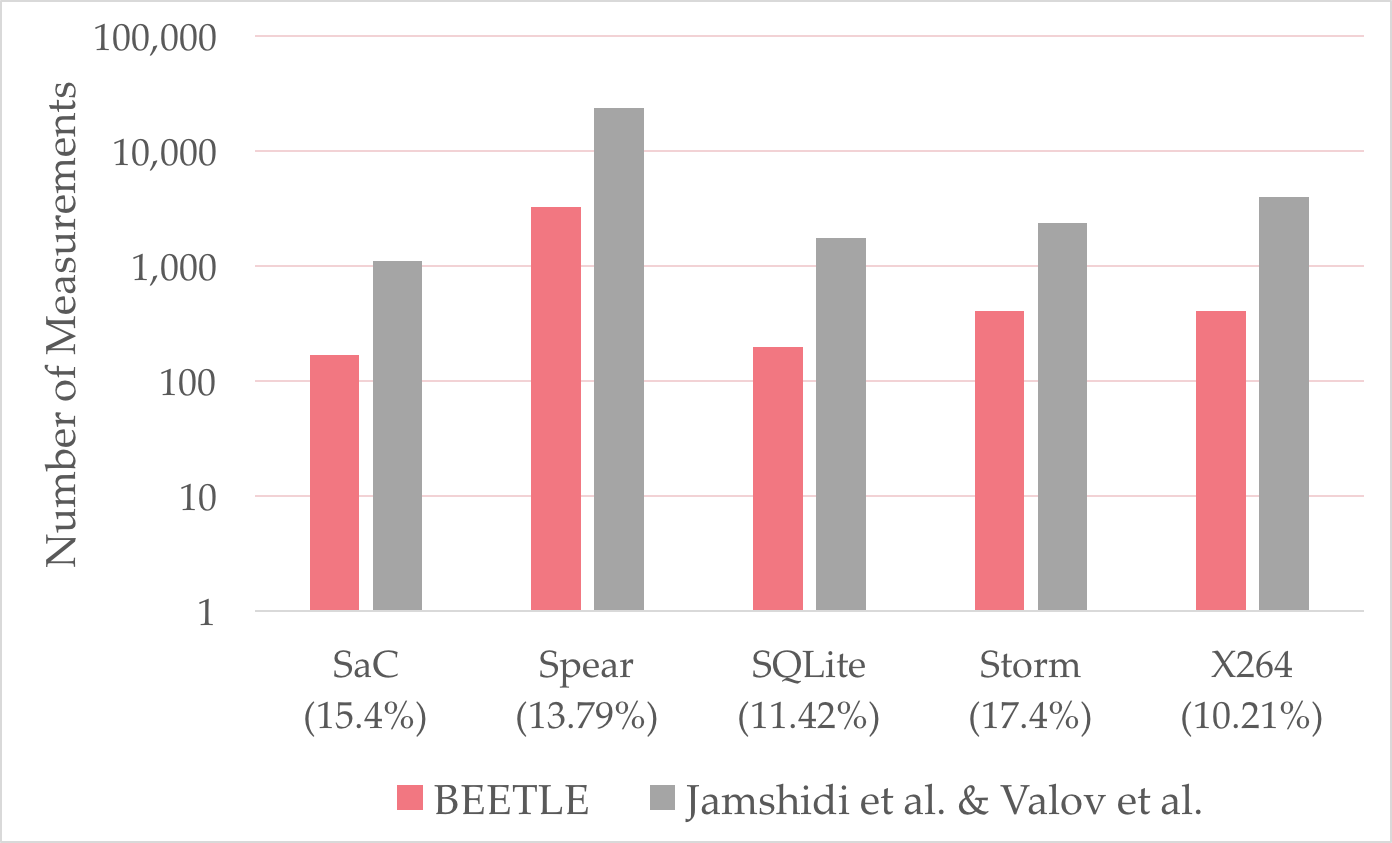
\includegraphics[width=0.95\linewidth]{figures/Measurements.png}
    \caption{{\small BEETLE v/s  state-of-the-art transfer learners. The numbers in parenthesis represent the numbers of measurements BEETLE uses in comparison to the  state-of-the-art learners.}}
    \label{fig:rq4_measurement}
\end{figure}


\section{Threats to Validity}
\label{sect:threats}
% \noindent{\em Reliability}:  care to either clearly define our
% algorithms or use implementations from the public domain
% (scikit-learn)~\cite{scikit-learn}. Also, all data and code used in this work are available on-line (\url{https://github.com/blinded4review}).

\noindent{\em External validity}: We selected a diverse set of subject systems and a large number of environment changes, but, as usual, one has to be careful when generalizing to other subject systems and environment changes. Even though we tried to run our experiment on a variety of software systems from different domains, we cannot generalize our results beyond these software systems.

% We performed experiments with more environmental changes and with additional measurements on the same subject systems (e.g., for SaC we also measured the time it takes to compile the program not only its execution), but we excluded those results because they were consistent with the presented data and did not provide additional insights. Even though we tried to run our experiment on a variety of software systems from different domains, we cannot generalize beyond these software systems. 

\noindent{\em Internal validity}: Due to the size of configuration spaces, we could only measure configurations exhaustively in one subject system (SPEAR) and had to rely on sampling (with substantial sampling size) for the others, which may miss effects in parts of the configuration space that we did not sample. We did not encounter any surprisingly different observation in our exhaustively measured {\sc SPEAR} dataset. Also, all other existing performance optimization work suffer from this threat.
Measurement noise in benchmarks can be reduced but not avoided. We performed benchmarks on dedicated systems and repeated each measurement three times. We repeated experiments when we encountered unusually large deviations.

\noindent{\em Parameter bias}: With all the transfer learners and predictors discussed here, there
are a number of internal parameters that have been set based on our engineering judgment. The result of changing these parameters may (or may not) have a significant impact on the outcomes of this study. To study the effect of these hyperparameters, we plot the trade-off between the hyperparameters (budget, lives) and NAR values (effectiveness) (see~\fig{tuning}). We note that the performance is correlated to the budget and number of lives, i.e., as the budget increases the NAR value decreases.


    
\section{Discussion}
\label{sect:disc}

\noindent\textbf{What is the effect of BEETLE on the day to day business of a software engineer?}
From an industrial perspective, 
BEETLE can be used in at least the following ways:
\begin{itemize}[leftmargin=*]
\item
Consider an organization which has to optimize their software system for different clients (who have different workload and hardware---different AWS subscriptions). While onboarding new clients, the company might not be able to afford to invest extensive resources in finding the near-optimal configuration to appease the client. State-of-the-art transfer learning techniques would expect the organization to provide a source workload (or environment) for this task. But without a  subject matter expert (SME) with the relevant knowledge, it is hard for humans to select a suitable source. \textit{BEETLE removes the need for such SMEs since it automates \underline{source selection}, along with transferring knowledge between the source and the target environment}.
\item
Consider an organization, which needs to migrate all their workload from a legacy platform to a different cloud platform (e.g., AWS to AZURE or vice versa). Such an organization now has many workloads that they need to optimize; however, they lack experience and performance measurements, on the new platform to accomplish this goal. \textit{In such cases, BEETLE provides a way to discover an ideal \underline{source} to transfer knowledge to enable efficient migration of workloads}. 
\end{itemize}

% \subsection{Does the (source) dataset matter?}

% \subsection{Does sample size of the bellwether dataset matter?}

% \subsection{Tradeoff between sample size (of bellwether) vs. ME?}

% For example, when we set the budget to 4\% of the total configuration space and lives = 4, we find the median NAR values found across all the subject system is 1.8.  We notice that as the budget increases the NAR values decreases and converges when the budget is 10\%. Note, this curve is an aggregate of the trade-off curves of all the software systems discussed in this paper. Since
% our objective is to minimize the number of measurements while reducing overall NAR, we assign the value of 5 to lives and 10\% to budget for our experiments.

% \noindent\textbf{When (not) to use bellwethers?}
% How to avoid negative transfer,in transfer learning, is an important open issue that is attracting much attention~\cite{gui2018negative, rosenstein2005transfer}. Negative transfer arises due to several factors such as incorrect source, noise in measurements, incorrect configuration options. In this work, bellwether effect can help overcome negative transfer caused due to incorrect source selection. However, this is not a comprehensive solution to address negative transfer in general. For other issues, just using bellwethers may not be adequate. 

% A point of caution: bellwether for a specific performance measure (such as latency) does not necessarily mean that it would be the bellwether for a different performance measure (such as throughput). During our experiments, we found that bellwether for latency does not work while optimizing throughput for {\sc Storm}. The reason for this is currently unknown and needs more exploration.

\begin{figure}[t]
    \centering
    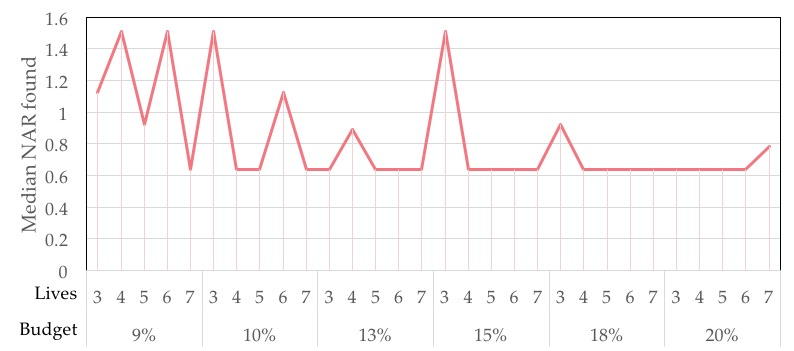
\includegraphics[width=0.98\linewidth, height=4cm]{figures/ParamTuning.jpg}
    \caption{The trade-off between the budget of the search, the number of lives, and the NAR (quality) of the solutions.}
    \label{fig:tuning}
\end{figure}


\noindent\textbf{Is BEETLE applicable in other domains?} In principle, yes. BEETLE could be applied to any transfer learning application, where the choice of the source data impacts the performance of transfer learning. This can be applied to problems such as configuring big data systems~\cite{JC:MASCOTS16}, finding suitable cloud configuration for a workload~\cite{Hsu2018scout, hsu2017low}, 
configuring hyperparameters of machine learning algorithms~\cite{fu2016tuning, fu2016differential, afridi2018}, runtime adaptation of robotic systems~\cite{jamshidi2017transfer}. In these applications, the correct choice of source datasets using bellwethers can help to reduce the amount of time it takes to discover a near-optimal configuration setting.

\noindent\textbf{Can BEETLE identify bellwethers in completely dissimilar environments?}
In theory, yes. Given a software system, BEETLE currently looks for an environment which can be used to find a near-optimal configuration for a majority of other environments for \textit{that} software system. Therefore, given performance measurements in a variety of environments, BEETLE can assist in discovering a suitable environment to transfer knowledge from. Our work shows that knowledge can be transferred between environments comprised of completely different hardware, software versions, and workloads.

\noindent\textbf{When are bellwethers ineffective?}
The existence of bellwethers depends on the following: 
\bi
\item
\textit{Metrics used:} Finding bellwether using metrics that are not justifiable, may be unsuccessful, for example, discovering bellwethers in performance optimization, by measuring MMRE instead of NAR may fail (see \url{http://tiny.cc/bw_metrics})~\cite{nair2017using}.
\item
\textit{Different Software System:} Bellwethers of a certain software system `A' may not work for software system `B.' In other words, it cannot be used for heterogeneous transfer learning.
\item
 \textit{Different Performance Measures: } Bellwether discovered for one performance measure (time) may not work for other performance measures (throughput).
\ei

\section{Related Work}
\label{sect:related}

% Performance optimization, also known as hyperparameter optimization, have gained attention due to ever increasing of highly-configurable systems~\cite{fu2016tuning, fu2016differential, tantithamthavorn2018impact}. %The significant portion of work in the machine learning domains namely Google Vizer~\cite{golovin2017google} (and in performance optimization~\cite{jamshidi2017transfer2, valov2017transferring}).

\noindent\textbf{Performance Optimization: }Modern software systems come with a large number of configuration options. 
For example, in {\sc Apache} (a popular web server) there are around 600 
different configuration options and in {\sc hadoop}, as of version 2.0.0, there are around 150 different configuration options, and the number of options is constantly growing~\cite{xu2015hey}. These configuration options control the 
internal 
properties of the system such as memory and response times. Given the large number of configurations, it becomes increasingly difficult to assess the impact of the configuration options on the system's performance. To address this issue, a common practice is to employ performance prediction models to estimate the performance of the system under these 
configurations~\cite{guo2013variability, hoste2006, hutter2014, thereska2010, 
valov2015, westermann12}. To leverage the full benefit of a software system and its features, researchers augment performance prediction models to enable
\textit{performance 
optimization}~\cite{nair2017using,oh2017finding}.
%Performance optimization 
%extends performance prediction by identifying the best set of configuration 
%options to accomplish a given task \textit{with near-optimal 
%performance}. 

Performance optimization is an important challenge in software engineering. As shown in the next few paragraphs, this problem has attracted much recent research interest. Approaches 
that use meta-heuristic 
search algorithms to explore the configuration space of Hadoop for high-performing configurations have been proposed~\cite{tang2018searching}. 
It has been reported that such meta-heuristic search can find configurations options that perform significantly better than baseline default configurations. 
In other work, a
control-theoretic framework called \textit{SmartConf} to automatically set and 
dynamically adjust performance-sensitive configurations to optimize 
configuration options~\cite{wang2018understanding}. For the specific case of 
deep learning clusters, a job scheduler called 
\textit{Optimus} has been developed to determine
configuration options that optimize training speed and resource 
allocations~\cite{peng2018optimus}. Performance optimization has also been extensively explored in other domains 
such as Systems Research~\cite{zhu2017bestconfig, li2018understanding} 
and Cloud Computing~\cite{alipourfard2017cherrypick, yadwadkar2017selecting, 
hsu2017low, Hsu2018scout, hsu2018micky}.

Much of the performance optimization tasks introduced above require access to measurements of the software system under various configuration settings. 
However, obtaining these performance measurements can cost a significant amount
of time and money. For example, in one of the software systems studied here ({\sc x264}), it takes over 1536 hours to obtain performance measurements for 11 out the 16 possible configuration options ~\cite{valov2017transferring}. This is in addition to other time-consuming tasks involved in commissioning these systems such as setup, 
tear down, etc. Further, making performance measurements can cost an exorbitant amount of money. In our case, for {\sc x264}, obtaining
performance measurements of 2048 configurations under different 
environments on Amazon AWS \texttt{c4.large} cluster cost us several thousand 
dollars.

\noindent\textbf{Transfer Learning: }
When a software system is deployed in a new environment, not every user can 
afford to repeat the costly process of building a new performance model to find 
an optimum configuration for that new environment. Instead, researchers propose 
the use of  transfer learning to 
reuse the measurements made for previous 
environments~\cite{valov2017transferring, jamshidi2017transfer, 
chen2011experience,golovin2017google}.
Jamshidi et al.~\cite{jamshidi2017transfer}, conducted a preliminary exploratory study of transfer learning in performance optimization to identify transferable knowledge between a source and a target environment, ranging from easily exploitable relationships to more subtle ones. 
They demonstrated that information about influential configuration options could 
be exploited in transfer learning and that knowledge about performance
behavior can be transferred between environments.

Following this, a number of transfer learning methods were developed to predict 
for the optimum configurations in a new \textit{target} environment, using the 
performance measures of another \textit{source} environment as a proxy. Several 
researchers have shown that transfer 
learning can decrease the cost of learning 
significantly~\cite{jamshidi2017transfer2,    valov2017transferring, 
jamshidi2017transfer,chen2011experience}.

All transfer learning methods place implicit faith in the quality of the source. A poor source can significantly deteriorate the performance of transfer learners. 


\noindent\textbf{Source Selection with Bellwethers: }
It is advised that the source used for transfer learning must be chosen with care to ensure optimum performance~\cite{yosinski2014transferable, 
long2015, afridi2018}. An incorrect choice of the source may result in the all too 
common \textit{negative transfer} 
phenomenon~\cite{afridi2018, ben2003, rosenstein2005,pan2010}. A negative transfer can be particularly damaging in that it often leads to performance 
degradation~\cite{jamshidi2017transfer2, afridi2018}. 
A preferred way to avoid negative transfer is with \textit{source 
selection}. Many methods have been proposed for identifying a suitable source for transfer learning~\cite{krishna18, krishna16, afridi2018}. Of these, source
selection using the bellwether effect is one of the simplest. It has been effective in several diverse domains of software engineering such as defect prediction, effort estimation, and code-smell detection~\cite{krishna18, 
mensah17a, 
mensah17b}. 

Besides negative transfer, previous approaches suffer from lack of scalability. For example, Google Visor~\cite{golovin2017google} Jamshidi et al.~\cite{jamshidi2017transfer} rely on a Gaussian process which known to   not scaling to large amounts of data in high dimensional spaces~\cite{rasmussen2004gaussian}
% \noindent\textbf{Negative Transfer.} The techniques proposed in the prior work implicitly assumes that the user would provide a good source to transfer knowledge. However, this is not always true, and an incorrect source can lead to Negative Transfer and hence return a sub-optimal configuration.
Accordingly, in this work, we introduce the notion of source selection with bellwether effect for transfer learning in performance optimization. With this, 
we develop a Bellwether Transfer Learner called BEETLE. We show that, for performance optimization, BEETLE can outperform both non-transfer and the transfer learning methods.    



\section{Conclusion}
\label{sect:conclusion}
Our approach exploits the bellwether effect---there are one or more bellwether environments which can be used to find good configurations for the rest of the environments. We also propose a new transfer learning method, called BEETLE, which exploits this phenomenon. As shown in this paper,  BEETLE can quickly identify the bellwether environments with only a few measurements ($\approx10\%$) and use it to find the near-optimal solutions in the target environments. Further, after extensive experiments with five highly configurable systems demonstrating, we show that  BEETLE:
\bi
\item Identifies   suitable sources to construct transfer learners;
\item Finds near-optimal configurations with only a small number of measurements ( $\le13.5\%\approx \frac{1}{7}^{th}$ of configuration space);
\item 
Performs as well as non-transfer learning approaches; and 
\item
Performs as well as state-of-the-art transfer learners.
\ei
Based on our experiments, we prove our initial hypothesis that: "whence to learn?" is an important question to answer and BEETLE can help answer this question effectively.

% We hence strongly endorse BEETLE for automatically configuring
% software when there exists numerous other variants of usage  executing
% in the target environment.
%As to future work, the findings of this paper allow for using

% \section*{ACKNOWLEDGEMENTS}
%  The work is partially funded by blinded for review. %by an NSF award \#1302169.


\bibliographystyle{IEEEtran}
\balance
\bibliography{bibliography} 
\end{document}

